% !BIB TS-program = biber

\RequirePackage[l2tabu,orthodox]{nag}

% TODO: decide if one-sided/two-sided
%\documentclass[headsepline,footsepline,footinclude=false,fontsize=11pt,paper=a4,listof=totoc,bibliography=totoc,BCOR=12mm,DIV=12]{scrbook} % two-sided
\documentclass[headsepline,footsepline,footinclude=false,oneside,fontsize=11pt,paper=a4,listof=totoc,bibliography=totoc]{scrbook} % one-sided

% TODO: change thesis information
\newcommand*{\getUniversity}{Technische Universität München}
\newcommand*{\getFaculty}{Informatics}
\newcommand*{\getDegree}{Informatics}
\newcommand*{\getSchool}{Computation, Information and Technology}
\newcommand*{\getTitle}{Analysis and Optimization of LLM Inference on Fast NVMe Storage}
\newcommand*{\getAuthor}{Ersjan Keri}
\newcommand*{\getDoctype}{Bachelor's Thesis}
\newcommand*{\getSupervisor}{Prof.\ Dr.\ Viktor Leis}
\newcommand*{\getAdvisor}{Gabriel Haas}
\newcommand*{\getKeywords}{LLM inference;Mixture of Experts;io\_uring;NVMe;memory hierarchy}
\newcommand*{\getSubmissionDate}{10.05.2026}
\newcommand*{\getSubmissionLocation}{Munich}

% TODO: change citation style in settings
\input{settings}

\begin{document}

% Set page numbering to avoid "destination with the same identifier has been already used" warning for cover page.
% (see https://en.wikibooks.org/wiki/LaTeX/Hyperlinks#Problems_with_Links_and_Pages).
\pagenumbering{alph}
\input{pages/cover}

\frontmatter{}

\input{pages/title}
\input{pages/disclaimer}
% Uncomment the following line if you want to include a software usage table (see example in pages/software_used.tex)
% \input{pages/software_used}
\addcontentsline{toc}{chapter}{Acknowledgments}
\thispagestyle{empty}

\vspace*{20mm}

\begin{center}
    {\usekomafont{sectioning}\usekomafont{section} Acknowledgments}
\end{center}

\vspace{10mm}

I am deeply grateful to my advisor, Gabriel Haas, whose guidance shaped this thesis from start to finish. He suggested the io\_uring direction during an early discussion about the page-fault path, and that single pointer defined the entire optimization chapter: the application-managed \texttt{O\_DIRECT} loader, the per-expert cache, the projection-group overlap, and the per-expert async dispatcher all descend from it. Beyond ideas, his careful reading and steady feedback across many iterations kept the work honest and the writing focused.

I thank my supervisor, Prof.\ Dr.\ Viktor Leis, for taking on the thesis.

I am grateful to the chair of Prof.\ Leis for providing the \texttt{cli-hiwi-02} server, arranged through Gabriel Haas, which hosted every cgroup sweep and every overnight run reported here; the AMD Ryzen~7 7700X and its two NVMe SSDs are the silent co-authors of every wall-clock number in the tables.

Finally, I thank my family for their patience through a project whose interesting moments were mostly invisible from the outside.

\cleardoublepage{}

\chapter{\abstractname}

A language model's weights are large arrays of numbers, called tensors, that the model multiplies on every generated token. The full set of tensors lives on disk in a single file, and the model runs fastest when the whole file is loaded into RAM. RAM has become expensive. DDR5 contract prices have roughly doubled since early 2025, and AI accelerator demand is forecast to consume about 20\% of global DRAM supply in 2026. NVMe SSDs are cheap and fast. Our goal is to extend llama.cpp so that a large model can run on a machine that does not have enough RAM to hold the whole model.

We started our analysis by building a tensor-level tracker that records, for every operation the model performs, which tensor it reads and which region of memory the data comes from. The trace shows that only 26.91\% of GPT-OSS-20B's weights and 7.69\% of GPT-OSS-120B's weights are read per generated token, because each Mixture-of-Experts layer activates only 4 of its 32 experts on 20B, and 4 of 128 on 120B. The inactive experts, which make up most of the model file, can stay on the SSD. Our backend pins the always-needed weights (the attention, output, and norm tensors) in RAM so the operating system cannot evict them, and prefetches the expert weights from the SSD asynchronously, overlapping the disk reads with the matrix multiplications that consume earlier reads. GPT-OSS-20B (12.85~GiB on disk) runs at 14.32 tokens per second on our test machine when the whole model fits in RAM. With limited RAM, where the model no longer fits, the default llama.cpp loader drops to 1.44 tokens per second. Our backend, on the same setting, runs the same model at 5.36 tokens per second. GPT-OSS-120B (60.88~GiB on disk) does not fit in the 30~GiB of RAM on our test machine at all. With limited RAM the default loader runs it at 4.96 tokens per second and our backend at 8.06 tokens per second.

\microtypesetup{protrusion=false}
\tableofcontents{}
\microtypesetup{protrusion=true}

\mainmatter{}

\chapter{Introduction}\label{chapter:introduction}

A modern language model's weights are tensors, large arrays of numbers that the model multiplies on every generated token.
The two models studied in this thesis, GPT-OSS-20B and GPT-OSS-120B~\cite{openai2025gptoss}, hold 12.85~GiB and 60.88~GiB of tensors on disk against the 30~GiB of RAM on our test machine.
The standard approach to inference, taken by llama.cpp~\cite{ggerganov2023llamacpp} among others, keeps the full set of model tensors resident in RAM throughout generation.
RAM has become an expensive resource: DDR5 contract prices have roughly doubled since early 2025~\cite{counterpoint_ddr5,networkworld_ddr5}, and AI accelerator demand is forecast to consume about 20\% of global DRAM supply in 2026~\cite{trendforce_dram2026}.
This thesis investigates inference under limited RAM, with the bulk of the model file left on the SSD.

We built a tensor-level tracer that records which tensors each operation accesses over the course of generation.
The trace shows that tensor access is not uniform.
The dense per-layer tensors (attention, output, and the norms) are read on every generated token.
The experts of each Mixture-of-Experts layer~\cite{shazeer2017moe}, which form the bulk of the model file, are not: a small router selects only a few of them per layer per token and the rest are skipped.
The dense tensors and the experts needed for one generated token together account for 26.91\% of GPT-OSS-20B and 7.69\% of GPT-OSS-120B.
Most of the model is therefore not needed at any one moment.

We pin the dense per-layer tensors in RAM so the kernel cannot evict them.
We manage the experts ourselves in a dedicated buffer that reads them from the SSD asynchronously.

We additionally built a small simulator that replays the trace under simple eviction strategies (LRU, LFU, and a frequency-with-decay variant) and reports the resulting hit rate of the buffer for a given number of expert slots.
The aim is to lay a foundation, not to design the best possible policy.
Every measurement runs inside a kernel-enforced memory limit set with Linux cgroups~\cite{cgroupv2}, so the available RAM is a hard, reproducible number rather than a condition that drifts between sessions.

With 7~GiB of RAM available, the default llama.cpp loader runs GPT-OSS-20B at 1.44 tokens per second.
Our backend runs it at 5.36 tokens per second, almost four times faster (\autoref{fig:headline}).
GPT-OSS-120B does not fit in 30~GiB of RAM at all.
The default loader runs it at 4.96 tokens per second.
Our backend runs it at 8.06 tokens per second.

\begin{figure}[htbp]
\centering
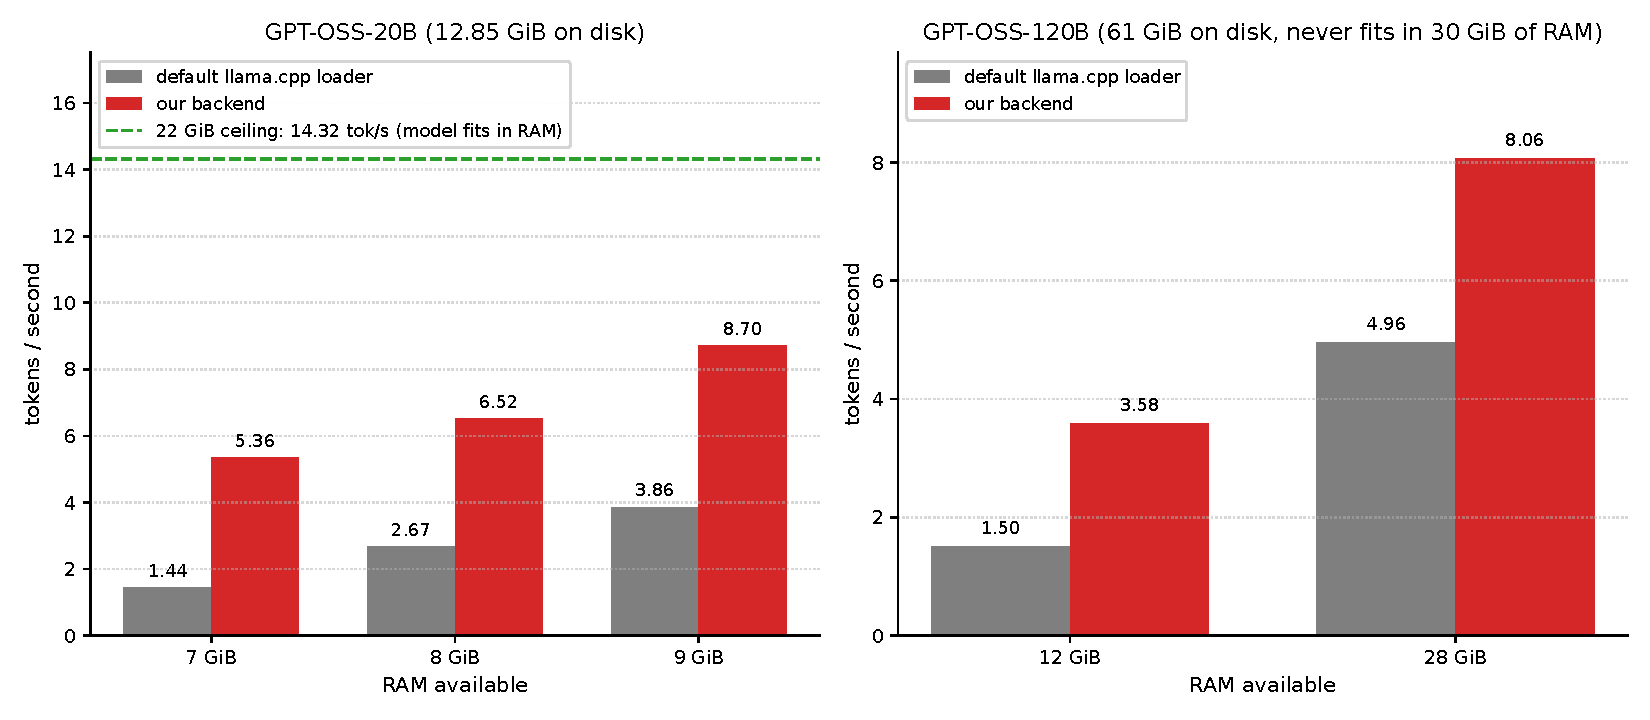
\includegraphics[width=0.85\textwidth]{figures/canon/headline.pdf}
\caption[Decode throughput of the default llama.cpp loader against our backend]{Decode throughput of the default llama.cpp loader (gray) against our backend (red), at three RAM caps for GPT-OSS-20B and two for GPT-OSS-120B. The dashed line on the left panel marks the 14.32~tok/s ceiling reached when GPT-OSS-20B fits entirely in RAM at the 22~GiB cap. GPT-OSS-120B (60.88~GiB on disk) never fits in the 30~GiB of RAM on the test machine, so there is no in-RAM ceiling on the right panel.}
\label{fig:headline}
\end{figure}

\chapter{Background}\label{chapter:background}

\section{Transformer Language Models}\label{sec:bg-transformer}

A transformer language model is a stack of layers~\cite{vaswani2017attention}.
Each layer applies two sub-blocks in sequence: a \emph{self-attention} block, in which each position attends to itself and earlier positions in the sequence, and a \emph{feed-forward network} (FFN), which transforms each token's representation independently.
GPT-OSS-20B has 24 such layers; GPT-OSS-120B has 36~\cite{openai2025gptoss}.

\begin{figure}[htbp]
\centering
\resizebox{0.55\textwidth}{!}{% Figure: high-level decoder-only transformer architecture, focused on one block.
% Goes in Chapter 2, Section 2.1 (Background / Transformer LLM Inference).
%
% Conventions:
%   * Pre-norm decoder block (RMSNorm before attention/FFN), as used by GPT-OSS
%   * Self-attention sub-block: black-boxed; refers to Eq. (attention)
%   * MoE FFN sub-block: highlighted in orange (matches the SSD-storage color
%     used for expert weights elsewhere); refers to Fig. (moe-ffn-dataflow)
%   * Residual connections drawn as green right-side loops
%   * x L badge indicates block stacking (L = 24 for GPT-OSS-20B, 36 for 120B)

\begin{tikzpicture}[
    font=\sffamily\small,
    >={Latex[length=2.5mm]},
    block/.style={
        draw, rectangle, rounded corners=1pt,
        minimum width=30mm, minimum height=8mm,
        align=center, font=\sffamily\small,
        fill=TUMAccentLightBlue!25,
    },
    norm/.style={block, fill=TUMLightGray!30, minimum width=24mm},
    moeblock/.style={
        block, fill=TUMAccentOrange!25, draw=TUMAccentOrange!75!black,
        font=\sffamily\bfseries\small,
    },
    plus/.style={
        draw, circle, fill=white, inner sep=0pt,
        minimum size=4mm, font=\small,
    },
    iolabel/.style={font=\sffamily\small\itshape, text=TUMDarkGray},
    arrow/.style={->, thick},
    residualstyle/.style={->, thick, draw=TUMAccentGreen!60!black},
    lbadge/.style={
        draw=TUMSecondaryBlue, fill=TUMAccentLightBlue!15,
        rounded corners=2pt, font=\sffamily\bfseries\small,
        text=TUMSecondaryBlue, inner sep=4pt,
    },
    xref/.style={font=\scriptsize\sffamily, anchor=west, inner sep=2pt},
]

  % --- Compressed input ---
  \node[iolabel, anchor=south] (inp) at (0, -1.0) {Embedding(tokens)};

  % --- One transformer block, bottom-up ---
  \node[norm]      (norm1) at (0, 0.5) {RMSNorm};
  \node[block]     (attn)  at (0, 1.9) {Self-Attention};
  \node[plus]      (plus1) at (0, 3.3) {$+$};
  \node[norm]      (norm2) at (0, 4.7) {RMSNorm};
  \node[moeblock]  (ffn)   at (0, 6.1) {MoE FFN};
  \node[plus]      (plus2) at (0, 7.5) {$+$};

  % --- Compressed output ---
  \node[iolabel, anchor=north] (out) at (0, 9.2) {RMSNorm $\to$ LM head $\to$ logits};

  % --- Vertical flow ---
  \draw[arrow] (inp)   -- (norm1);
  \draw[arrow] (norm1) -- (attn);
  \draw[arrow] (attn)  -- (plus1);
  \draw[arrow] (plus1) -- (norm2);
  \draw[arrow] (norm2) -- (ffn);
  \draw[arrow] (ffn)   -- (plus2);
  \draw[arrow] (plus2) -- (out);

  % --- Residual loops (right side) ---
  \draw[residualstyle] (0, -0.3) -- (2.4, -0.3) -- (2.4, 3.3) -- (plus1);
  \draw[residualstyle] (0,  3.9) -- (2.4,  3.9) -- (2.4, 7.5) -- (plus2);

  % --- Block boundary ---
  \begin{scope}[on background layer]
    \node[
      draw=TUMGray, dashed, rounded corners=2pt,
      fit=(norm1) (plus2),
      inner xsep=8mm, inner ysep=4mm,
    ] (blockbox) {};
  \end{scope}

  % --- x L badge (left of block boundary) ---
  \node[lbadge, anchor=east] at ($(blockbox.west) + (-0.2, 0)$) {$\times\, L$};

  % --- Cross-references on the right ---
  \node[xref, text=TUMAccentOrange!85!black] at (3.0, 6.1) {See Fig.~\ref{fig:moe-ffn-dataflow}};

  % --- Residual color key ---
  \node[xref, text=TUMAccentGreen!60!black, anchor=west] at (3.0, 4.7) {residual};

\end{tikzpicture}
}
\caption[Decoder-only transformer block]{One transformer layer. Self-attention and the feed-forward network are applied in sequence with residual connections; the model is a stack of $L$ such layers ($L=24$ for GPT-OSS-20B, $L=36$ for GPT-OSS-120B) followed by a final norm and the output projection.}
\label{fig:transformer-block}
\end{figure}

Generating text happens in two phases.
The first, called \emph{prefill}, processes the entire prompt.
The second, called \emph{decode}, produces one new token at a time, each appended to the input for the next step.
Our throughput metric counts tokens generated per second during decode.

To avoid recomputing attention over all prior tokens at every decode step, each layer caches its key and value tensors.
We call this the \emph{KV cache}.
GPT-OSS interleaves layers using a 128-token sliding window with layers using full attention~\cite{openai2025gptoss}, but the KV cache is allocated up front for the full configured 131072-token context.
It therefore reserves 3.02~GiB of RAM on GPT-OSS-20B and 4.53~GiB on GPT-OSS-120B regardless of how many tokens are actually generated.


\section{Mixture-of-Experts}\label{sec:bg-moe}

In a Mixture-of-Experts layer, the FFN is replaced by many small subnetworks, called \emph{experts}~\cite{shazeer2017moe}.
For each generated token, a small \emph{router} selects only a few of them, and the rest are not read.
GPT-OSS-20B has 32 experts per layer and selects 4; GPT-OSS-120B has 128 experts per layer and also selects 4~\cite{openai2025gptoss}.

Each expert is three weight matrices, called the \emph{up}, \emph{gate}, and \emph{down} projections.
We call each of these matrices a \emph{slice}.
A slice is 4.20~MiB on disk on both GPT-OSS models (4{,}406{,}400 bytes).
One MoE layer therefore reads $4 \times 3 = 12$ slices per generated token.
Across the 24 layers of GPT-OSS-20B that is 288 slices per token, 1.18~GiB of weight data.
On GPT-OSS-120B it is $4 \times 3 \times 36 = 432$ slices, 1.77~GiB.

\begin{figure}[htbp]
\centering
\resizebox{0.95\textwidth}{!}{% Figure: MoE-FFN dataflow for one decode token, GPT-OSS-MoE / llama.cpp.
% Goes in Chapter 2 (background).
%
% Architecture-only view: what is computed, with what shapes, in what order,
% for one decode token at one MoE layer. Independent of weight residency.
%
% Conventions (also used by the timing variants in Chapter 7):
%   * activations  : light blue tiles
%   * expert weights (live on SSD, must be loaded): red tiles
%   * compute ops  : green rounded boxes
%   * routing      : violet rounded box
%
% Anchored facts (verified empirically against
% tensor-tracing/desktopui/data/memory-map.json):
%   d := n_embd = ffn_dim = 2880    (GPT-OSS-20B and -120B)
%   k := n_expert_used = 4 (top-k routing)
%   n_e := n_expert = 32 (20B), 128 (120B)
%   per-expert per-projection slice = 2880 * 2880 weights, MXFP4 = 4.20 MiB on disk
%   SwiGLU-OAI: alpha = 1.702, limit = 7.0    (llama-graph.cpp:1764-1765)

\begin{tikzpicture}[
  x=1mm, y=1mm,
  font=\footnotesize,
  every node/.style={inner sep=1pt, outer sep=0pt},
  act/.style    ={draw=blue!55!black,   fill=blue!10,    line width=0.4pt, rounded corners=0.6pt, align=center, font=\scriptsize},
  weight/.style ={draw=red!55!black,    fill=red!12,     line width=0.4pt, rounded corners=0.6pt, align=center, font=\scriptsize},
  op/.style     ={draw=green!55!black,  fill=green!12,   line width=0.5pt, rounded corners=1.2pt, align=center, font=\scriptsize},
  router/.style ={draw=violet!55!black, fill=violet!12,  line width=0.5pt, rounded corners=1.2pt, align=center, font=\scriptsize},
  flow/.style       ={->, >={Stealth[length=1.5mm]}, line width=0.4pt, draw=black!75},
  smallflow/.style  ={->, >={Stealth[length=1.0mm]}, line width=0.3pt, draw=black!60},
  panel/.style      ={draw=black!35, dashed, line width=0.35pt, rounded corners=1.2pt},
  expicon/.style    ={draw=black!50, fill=gray!8, line width=0.3pt, rounded corners=0.6pt, align=center, font=\scriptsize},
]

  % ============================================================
  % FIGURE TITLE: name the operation
  % Centred on image center x=60 (where y[1,d] also lives, at the bottom).
  % ============================================================
  \node[anchor=south, font=\small\bfseries] at (60, 136)
        {Mixture-of-Experts FFN block};
  \node[anchor=south, font=\scriptsize\itshape, text=black!65] at (60, 132)
        {one decode token, one layer; $k\!=\!4$ of $n_e\!=\!32$ experts activated};

  % ============================================================
  % HEADER ROW: input vector x (centred on x=60 so it sits directly above y)
  % ============================================================
  \node[act, minimum width=22mm, minimum height=4mm] (x) at (60, 124)
        {$\mathbf{x}\,[1,d]$};

  % ============================================================
  % ROUTER block (centred on x=60)
  % ============================================================
  \node[router, minimum width=46mm, minimum height=10mm] (router) at (60, 114)
        {\textbf{Router}\\[0.2ex]\scriptsize linear\,$\mathbf{x}\!\cdot\!\mathbf{W}_{r}$
         $\to$\,softmax $\to$ top-$k$};
  \draw[flow] (x) -- (router);

  \node[weight, minimum width=18mm, minimum height=4mm, font=\tiny] (Wr) at (95, 114)
        {$\mathbf{W}_{r}\,[d,n_e]$};
  \draw[smallflow] (Wr) -- (router);

  % Router outputs: placed symmetrically around x=60 (centres at 38 and 82
  % so the section is balanced on the figure's vertical centerline).
  \node[act, minimum width=34mm, minimum height=6mm] (sel) at (38, 102)
        {selected\_experts\,$[k]$\\[-0.4ex]\scriptsize\texttt{[5,\,12,\,23,\,31]}};
  \node[act, minimum width=40mm, minimum height=6mm] (rw) at (82, 102)
        {router\_weights\,$[k]$\\[-0.4ex]\scriptsize\texttt{[0.31,\,0.27,\,0.24,\,0.18]}};

  \draw[flow] (router.south) -| (sel.north);
  \draw[flow] (router.south) -| (rw.north);

  % ============================================================
  % CALLOUT: expert e = 0 in detail.
  % Layout intent (mirrors what each operation actually consumes):
  %   y=82  Wg | x | Wu          three inputs to the gate/up step
  %   y=70  gate matmul | up matmul        parallel matmuls
  %   y=62  gate_0 | up_0                 their two outputs
  %   y=52  swiglu(gate_0, up_0)          combiner
  %   y=42  act_0 | Wd                    two inputs to the down step
  %   y=30  down matmul                   single matmul
  %   y=22  down_0                        per-expert contribution
  % ============================================================
  \draw[panel] (-2, 16) rectangle (60, 88);
  % Title placed ABOVE the panel so it labels the box rather than living inside it.
  \node[anchor=south west, font=\scriptsize\itshape, text=black!65]
        at (-2, 89) {Detail of one expert (representative; \,$e\!=\!0$)};

  % --- top row: parallel inputs to gate/up ---
  \node[weight, minimum width=18mm, minimum height=4mm] (Wg0) at (14, 82)
        {$\mathbf{W}_{g}^{[0]}\,[d,d]$};
  \node[act,    minimum width=10mm, minimum height=4mm] (x0)  at (29, 82)
        {$\mathbf{x}\,[1,d]$};
  \node[weight, minimum width=18mm, minimum height=4mm] (Wu0) at (44, 82)
        {$\mathbf{W}_{u}^{[0]}\,[d,d]$};

  % --- gate / up matmul nodes (green box = "compute op", no need to label "matmul") ---
  \node[op, minimum width=18mm, minimum height=7mm, font=\footnotesize] (gate0) at (14, 70)
        {$\mathbf{x}\!\cdot\!\mathbf{W}_{g}^{[0]\!\top}$};
  \node[op, minimum width=18mm, minimum height=7mm, font=\footnotesize] (up0)   at (44, 70)
        {$\mathbf{x}\!\cdot\!\mathbf{W}_{u}^{[0]\!\top}$};

  % straight feeders Wg -> gate, Wu -> up
  \draw[smallflow] (Wg0) -- (gate0);
  \draw[smallflow] (Wu0) -- (up0);
  % x feeds BOTH gate and up (this is the parallelism the figure makes visible)
  \draw[smallflow] (x0.south) to[out=-90, in=60]  (gate0.north east);
  \draw[smallflow] (x0.south) to[out=-90, in=120] (up0.north west);

  % --- gate / up output activations ---
  \node[act, minimum width=18mm, minimum height=4mm] (g0) at (14, 62) {gate$_{0}\,[1,d]$};
  \node[act, minimum width=18mm, minimum height=4mm] (u0) at (44, 62) {up$_{0}\,[1,d]$};
  \draw[smallflow] (gate0) -- (g0);
  \draw[smallflow] (up0)   -- (u0);

  % --- swiglu combiner (consumes both) ---
  \node[op, minimum width=54mm, minimum height=8mm, font=\footnotesize] (sw0) at (29, 52)
        {$\mathrm{swiglu}(\,\mathrm{gate}_{0}[1,d],\;\mathrm{up}_{0}[1,d]\,)$};
  \draw[smallflow] (g0) -- ([xshift=-7mm]sw0.north);
  \draw[smallflow] (u0) -- ([xshift= 7mm]sw0.north);

  % --- act_0 (left) and Wd (right) on the SAME row, both feeding the down matmul ---
  \node[act,    minimum width=18mm, minimum height=4mm] (a0)  at (15, 42)
        {act$_{0}\,[1,d]$};
  \node[weight, minimum width=18mm, minimum height=4mm] (Wd0) at (43, 42)
        {$\mathbf{W}_{d}^{[0]}\,[d,d]$};
  % swiglu output funnels into act_0 (curving left so it ends pointing into a0)
  \draw[smallflow] (sw0.south) to[out=-90, in=80] (a0.north);

  % --- down matmul (single, takes act_0 and Wd as inputs) ---
  \node[op, minimum width=22mm, minimum height=7mm, font=\footnotesize] (down0) at (29, 30)
        {$\mathrm{act}_{0}\!\cdot\!\mathbf{W}_{d}^{[0]\!\top}$};
  \draw[smallflow] (a0.south)  to[out=-90, in=120] (down0.north west);
  \draw[smallflow] (Wd0.south) to[out=-90, in=60]  (down0.north east);

  % --- down output tile (the per-expert contribution from e=0) ---
  \node[act, minimum width=22mm, minimum height=4mm] (do0) at (29, 22)
        {down$_{0}\,[1,d]$};
  \draw[smallflow] (down0) -- (do0);

  % ============================================================
  % EXPERT ICONS for e = 1, 2, 3 to the right of the callout.
  % Each icon has the SAME outer height as the dashed callout (y in [16, 88])
  % and is wide enough that "down_i [1,d]" fits without clipping.
  % Element ordering inside an icon mirrors the detail panel exactly.
  % ============================================================
  \begin{scope}[shift={(72, 0)}]
    % Single header above the whole 3-icon row (placed once, not per-box)
    \node[anchor=south west, font=\scriptsize\itshape, text=black!65] at (-10, 89)
          {Other experts (same structure, same compute):};

    \foreach \i/\eid in {1/12, 2/23, 3/31} {
      \pgfmathsetmacro{\xi}{(\i-1)*22}
      % Outer icon box: height matches callout (72 mm), width 20 mm
      \node[expicon, minimum width=20mm, minimum height=72mm, anchor=north]
            (e\i) at (\xi, 88) {};
      % Header on a SINGLE row: "e=i (eid=N)"
      \node[anchor=north, font=\scriptsize, text=black!85]
            at (\xi, 86) {$e\!=\!\i$\;\textit{(eid=\eid)}};
      % Vertical stack mirroring the callout: Wg, Wu, gate, up, swiglu,
      % Wd, down, then the down_i output tile separated at the bottom.
      \node[weight, minimum width=15mm, minimum height=4mm, font=\scriptsize] at (\xi, 78) {$\mathbf{W}_{g}^{[\i]}$};
      \node[weight, minimum width=15mm, minimum height=4mm, font=\scriptsize] at (\xi, 72) {$\mathbf{W}_{u}^{[\i]}$};
      \node[op,     minimum width=15mm, minimum height=4mm, font=\scriptsize] at (\xi, 66) {gate};
      \node[op,     minimum width=15mm, minimum height=4mm, font=\scriptsize] at (\xi, 60) {up};
      \node[op,     minimum width=15mm, minimum height=4mm, font=\scriptsize] at (\xi, 54) {swiglu};
      \node[weight, minimum width=15mm, minimum height=4mm, font=\scriptsize] at (\xi, 46) {$\mathbf{W}_{d}^{[\i]}$};
      \node[op,     minimum width=15mm, minimum height=4mm, font=\scriptsize] at (\xi, 40) {down};
      \node[act,    minimum width=17mm, minimum height=4mm, font=\scriptsize, inner sep=0.7pt]
            (di\i_local) at (\xi, 28) {down$_{\i}\,[1,d]$};
    }
  \end{scope}

  % (Routing dashed arrows removed: selected_experts feeding the four expert
  % blocks and router_weights feeding the weighted sum are obvious from the
  % spatial layout; the arrows added clutter without information.)

  % ============================================================
  % WEIGHTED SUM BAND
  % ============================================================
  % Down output tiles in a row above the weighted-sum op
  % (down_0 already drawn inside the callout at (20, 22). The icons drew
  % down_1..down_3 inside their boxes at local x=70..100, y=41.5.)

  \node[op, minimum width=120mm, minimum height=10mm, font=\footnotesize] (sum) at (60, 9)
        {\textbf{Weighted sum:}\;\;
         $\mathbf{y} \;=\; \sum_{e=0}^{k-1}\;\mathrm{router\_weights}[e]\,\cdot\,\mathrm{down}_{e}
         \quad\to\quad [1,d]$};

  % connectors from each down_i into the sum (vertical drops onto sum.north)
  \draw[smallflow] (do0.south) -- ([xshift=-31mm]sum.north);
  \draw[smallflow] (72,  26) -- ([xshift=12mm]sum.north);
  \draw[smallflow] (94,  26) -- ([xshift=34mm]sum.north);
  \draw[smallflow] (116, 26) -- ([xshift=56mm]sum.north);

  % (router_weights -> Weighted sum dashed arrow removed; the formula inside
  % the sum block already states the dependence explicitly.)

  % ============================================================
  % FINAL OUTPUT (lowered slightly so the sum -> y arrow has the same visible
  % length as the x -> Router arrow at the top of the figure)
  % ============================================================
  \node[act, minimum width=22mm, minimum height=4mm] (y) at (60, -1)
        {$\mathbf{y}\,[1,d]$};
  \draw[flow] (sum) -- (y);
  \node[anchor=west, font=\scriptsize\itshape, text=black!65] at (75, -1)
        {to residual\,+\,RMSNorm\,+\,next layer};

  % ============================================================
  % LEGEND (right column, well separated)
  % ============================================================
  \begin{scope}[shift={(132, 110)}, font=\scriptsize]
    \node[anchor=west, font=\scriptsize\bfseries] at (0, 6) {Legend};
    \node[act,    minimum width=8mm, minimum height=3mm] at (4, 0)   {};
      \node[anchor=west] at (8.5, 0)   {activation tile};
    \node[weight, minimum width=8mm, minimum height=3mm] at (4, -5)  {};
      \node[anchor=west] at (8.5, -5)  {expert weight (on SSD)};
    \node[op,     minimum width=8mm, minimum height=3mm] at (4, -10) {};
      \node[anchor=west] at (8.5, -10) {compute op};
    \node[router, minimum width=8mm, minimum height=3mm] at (4, -15) {};
      \node[anchor=west] at (8.5, -15) {routing};

    % Footnote, well below the swatches so no overlap
    \node[anchor=north west, font=\tiny\itshape, text=black!65,
          align=left, text width=42mm] at (0, -22)
         {Red tiles live on SSD; how and when each is loaded is the subject
          of \autoref{chapter:implementation}.};
  \end{scope}

\end{tikzpicture}
}
\caption[Mixture-of-Experts layer for one generated token]{One MoE layer applied to one generated token. The router selects 4 of the 32 experts (highlighted in red); the remaining 28 are not read. Each selected expert applies its three weight matrices (up, gate, down), and the four expert outputs are combined into the layer output.}
\label{fig:moe-ffn-dataflow}
\end{figure}


\section{How llama.cpp Loads Weights}\label{sec:bg-llamacpp}

llama.cpp~\cite{ggerganov2023llamacpp} stores model files in GGUF, a single-file binary format whose header lists each tensor's name, shape, type, and offset, followed by the tensor data~\cite{gguf_spec}.

The default loader maps the file into the process's virtual address space with \texttt{mmap}~\cite{mmap_man}, so tensor bytes are read by dereferencing pointers.
A first access to a not-yet-resident page triggers a \emph{page fault}: the kernel suspends the thread, reads the page (and a small readahead window around it, on the order of tens of KiB) from disk into the \emph{page cache}, maps it at the faulting address, and resumes the thread.
Subsequent accesses to the same page return without entering the kernel.
The page cache lives in kernel-managed memory, and the kernel chooses which pages to evict when other allocations need the space.


\section{Asynchronous Disk I/O on Linux}\label{sec:bg-iouring}

\texttt{io\_uring} is a Linux kernel interface for asynchronous I/O~\cite{axboe2019iouring}.
The application and the kernel share submission and completion queues in memory: a \emph{submission queue} (SQ), into which the application writes read requests, and a \emph{completion queue} (CQ), into which the kernel writes results.
A single \texttt{io\_uring\_enter} system call notifies the kernel that new submission entries are pending. The kernel reads them in place from shared memory and dispatches the I/O without blocking the calling thread.
Each completion entry carries a user-supplied tag that identifies the request it satisfies, so the application can match completions to requests and drain the queue at its own pace.

\texttt{O\_DIRECT} is an \texttt{open(2)} flag that tells the kernel to bypass the page cache for that file~\cite{open_man}.
On a read, the kernel programs the device to DMA the data directly into the application-supplied buffer with no copy through the page cache.
The cost is a strict alignment contract: file offset, read length, and destination buffer address must all be multiples of the device's logical block size, which is 512 bytes on the NVMe used here~\cite{nvme_spec}.
The two features are orthogonal: \texttt{io\_uring} can serve cached or direct I/O, and \texttt{O\_DIRECT} can be used with synchronous \texttt{read(2)} as well.

Combining the two moves both the buffer and the eviction decision into the application.
The submission and completion queues are mmap'd into the application's address space at \texttt{io\_uring} setup time, so the application writes submissions and reads completions without entering the kernel except for the one \texttt{io\_uring\_enter} call per batch.
The data buffer is allocated by the application and is the DMA target (\autoref{fig:iouring-read}).
With no page cache between the device and the buffer, there is no kernel-side cache to evict from; if the application keeps a fixed-size pool of buffer slots, eviction is its responsibility (\autoref{fig:iouring-evict}).

\begin{figure}[htbp]
\centering
\resizebox{0.95\textwidth}{!}{% Figure 2.3: read flow under io_uring + O_DIRECT.
% Goes in Chapter 2, Section 2.4. Companion figure (eviction) lives in
% figures/io_uring_evict.tex with the same column layout.
%
% Three columns, identical placement to the eviction figure:
%   Application (left, dashed): SQ ring, CQ ring, buffer of N=5 slots
%   Kernel       (mid, solid) : single rounded box
%   NVMe SSD    (right, solid): single rounded box
%
% Three arrows distinguished by what they actually carry:
%   (orange, syscall)       app -> kernel: io_uring_enter notifies the kernel
%                           that new SQEs are queued. SQEs themselves stay in
%                           the SQ ring, which the kernel reads in place.
%   (green, metadata)       kernel -> CQ: the kernel writes one CQE per read.
%                           A CQE is a (tag, status) record, not data.
%   (blue, data)            NVMe -> free buffer slot: O_DIRECT DMA. This is
%                           the only arrow on this figure that moves bytes
%                           of file content.
%
% Dashed gray "buffer ptr" link from SQE to the destination buffer slot
% answers "how does io_uring know where to write": each SQE carries a
% pointer to the target buffer slot.
%
% A small italic note under the CQ row reinforces that CQEs carry only
% tag + status (no data flows through the CQ).

\begin{tikzpicture}[
    font=\sffamily\small,
    >={Latex[length=2.5mm]},
    sqe/.style={draw=TUMBlue, fill=TUMBlue!15, minimum width=8mm, minimum height=6mm, font=\footnotesize, inner sep=1pt},
    cqe/.style={draw=TUMAccentGreen!80!black, fill=TUMAccentGreen!25, minimum width=8mm, minimum height=6mm, font=\footnotesize, inner sep=1pt},
    bufslot/.style={draw=TUMSecondaryBlue, fill=TUMAccentLightBlue!40, minimum width=10mm, minimum height=6mm, font=\footnotesize, inner sep=1pt},
    bigbox/.style={draw=TUMGray, rounded corners=2pt, minimum width=2.0cm, font=\small\bfseries},
    arrow/.style={->, thick},
    arrowlbl/.style={font=\scriptsize, sloped=false},
    annot/.style={font=\scriptsize\itshape, text=TUMDarkGray},
]

  % --- Application column ---
  \node[font=\small\bfseries, anchor=west] (applabel) at (0.2, 5.0) {Application};

  \node[anchor=east, font=\footnotesize] (sqlabel) at (0.7, 4.1) {SQ};
  \node[sqe, anchor=west] (s0) at (0.8, 4.1) {S\textsubscript{0}};
  \node[sqe, anchor=west] (s1) at (s0.east) {S\textsubscript{1}};
  \node[sqe, anchor=west] (s2) at (s1.east) {S\textsubscript{2}};
  \node[sqe, anchor=west] (s3) at (s2.east) {S\textsubscript{3}};
  \node[sqe, anchor=west, draw=TUMBlue!50, fill=white] (s4) at (s3.east) {};

  \node[anchor=east, font=\footnotesize] (cqlabel) at (0.7, 3.0) {CQ};
  \node[cqe, anchor=west] (c0) at (0.8, 3.0) {C\textsubscript{0}};
  \node[cqe, anchor=west] (c1) at (c0.east) {C\textsubscript{1}};
  \node[cqe, anchor=west] (c2) at (c1.east) {C\textsubscript{2}};
  \node[cqe, anchor=west] (c3) at (c2.east) {C\textsubscript{3}};
  \node[cqe, anchor=west, draw=TUMAccentGreen!50, fill=white] (c4) at (c3.east) {};

  % CQ contents annotation
  \node[annot, anchor=north west] (cqannot)
      at ($(c0.south west)+(0,-0.5mm)$) {each CQE: (tag, bytes read), no data};

  \node[anchor=east, font=\footnotesize] (buflabel) at (0.7, 1.5) {buffer};
  \node[bufslot, anchor=west] (b0) at (0.8, 1.5) {slice\textsubscript{0}};
  \node[bufslot, anchor=west] (b1) at (b0.east) {slice\textsubscript{1}};
  \node[bufslot, anchor=west] (b2) at (b1.east) {slice\textsubscript{2}};
  \node[bufslot, anchor=west] (b3) at (b2.east) {slice\textsubscript{3}};
  \node[bufslot, anchor=west, draw=TUMSecondaryBlue!60, fill=TUMAccentLightBlue!10] (bfree) at (b3.east) {free};

  \begin{scope}[on background layer]
    \node[draw=TUMGray, dashed, rounded corners=2pt, fit=(applabel) (sqlabel) (s4) (cqlabel) (c4) (cqannot) (buflabel) (bfree), inner sep=4mm] (appbox) {};
  \end{scope}

  % --- Kernel column ---
  \node[bigbox, fill=TUMLightGray!25, minimum height=3.4cm, anchor=center] (kernel) at (9.6, 3.0) {Kernel};

  % --- NVMe column ---
  \node[bigbox, fill=TUMLightGray!50, minimum height=1.4cm, draw=TUMBlack, anchor=center] (nvme) at (12.6, 1.5) {NVMe};

  % --- Active arrows ---
  % (orange) io_uring_enter is a syscall notifying the kernel.
  % SQEs stay in shared memory; the kernel reads them in place.
  \draw[arrow, TUMAccentOrange]
      (s4.east) -- node[arrowlbl, above] {\texttt{io\_uring\_enter} (syscall)}
      (kernel.west |- s2);

  % (green) kernel writes a CQE into shared memory: tag + status only.
  \draw[arrow, TUMAccentGreen!60!black]
      (kernel.west |- c2) -- node[arrowlbl, above] {write CQE}
      (c4.east);

  % (blue, thicker) DMA: NVMe writes file bytes directly into the free
  % buffer slot, bypassing the kernel column. This is the only arrow on
  % this figure that carries data.
  \draw[arrow, TUMSecondaryBlue, line width=1pt]
      (nvme.west) -- node[arrowlbl, above] {data (DMA, \texttt{O\_DIRECT})}
      (bfree.east);

\end{tikzpicture}
}
\caption[Read flow under \texttt{io\_uring} with \texttt{O\_DIRECT}]{Read flow under \texttt{io\_uring} combined with \texttt{O\_DIRECT}. The submission queue, completion queue, and the data buffer all live in the application's address space. Each SQE carries the destination buffer pointer for its read. One \texttt{io\_uring\_enter} system call (orange) notifies the kernel; the kernel reads the SQEs from shared memory, pins the destination pages, and programs the device. The device then DMAs the file bytes into the destination, overwriting whatever was there (blue): this is the only path on the figure that carries data. The kernel writes one CQE per read into the CQ ring (green); a CQE is a (tag, bytes-read) record only, no data. The application reads the CQ in place without another syscall.}
\label{fig:iouring-read}
\end{figure}

\begin{figure}[htbp]
\centering
\resizebox{0.95\textwidth}{!}{% Figure 2.4: eviction step under io_uring + O_DIRECT.
% Same column placement and same building blocks as figure 2.3
% (figures/io_uring_rings.tex) so the two figures contrast cleanly.
%
% On a cache miss with the buffer already full, the application picks a
% victim slot under its replacement policy (LRU, LFU, or LFU-aging in our
% backend). The miss is then served by the same SQ -> io_uring_enter ->
% DMA -> CQ flow shown in figure 2.3, with the freshly freed slot as the
% DMA target. Eviction itself is purely application-internal: no syscall,
% no device traffic.
%
% Active arrow on this figure:
%   (red)    application policy marks slice_3 as the victim slot
% Inactive arrows:
%   (gray, dashed) the io_uring rings and DMA path drawn in light gray to
%                  show the same building blocks are still in place.

\begin{tikzpicture}[
    font=\sffamily\small,
    >={Latex[length=2.5mm]},
    sqe/.style={draw=TUMBlue!40, fill=TUMBlue!8, minimum width=8mm, minimum height=6mm, font=\footnotesize, inner sep=1pt, text=TUMDarkGray},
    cqe/.style={draw=TUMAccentGreen!40, fill=TUMAccentGreen!10, minimum width=8mm, minimum height=6mm, font=\footnotesize, inner sep=1pt, text=TUMDarkGray},
    bufslot/.style={draw=TUMSecondaryBlue, fill=TUMAccentLightBlue!40, minimum width=10mm, minimum height=6mm, font=\footnotesize, inner sep=1pt},
    bigbox/.style={draw=TUMGray, rounded corners=2pt, minimum width=2.0cm, font=\small\bfseries},
    arrow/.style={->, thick},
    arrowlbl/.style={font=\scriptsize, sloped=false},
    inactive/.style={draw=TUMGray!50, dashed, ->, thick},
]

  % --- Application column (dashed border) ---
  \node[font=\small\bfseries, anchor=west] (applabel) at (0.2, 5.0) {Application};

  \node[anchor=east, font=\footnotesize] (sqlabel) at (0.7, 4.1) {SQ};
  \node[sqe, anchor=west] (s0) at (0.8, 4.1) {};
  \node[sqe, anchor=west] (s1) at (s0.east) {};
  \node[sqe, anchor=west] (s2) at (s1.east) {};
  \node[sqe, anchor=west] (s3) at (s2.east) {};
  \node[sqe, anchor=west] (s4) at (s3.east) {};

  \node[anchor=east, font=\footnotesize] (cqlabel) at (0.7, 3.0) {CQ};
  \node[cqe, anchor=west] (c0) at (0.8, 3.0) {};
  \node[cqe, anchor=west] (c1) at (c0.east) {};
  \node[cqe, anchor=west] (c2) at (c1.east) {};
  \node[cqe, anchor=west] (c3) at (c2.east) {};
  \node[cqe, anchor=west] (c4) at (c3.east) {};

  \node[anchor=east, font=\footnotesize] (buflabel) at (0.7, 1.5) {buffer};
  \node[bufslot, anchor=west] (b0) at (0.8, 1.5) {slice\textsubscript{0}};
  \node[bufslot, anchor=west] (b1) at (b0.east) {slice\textsubscript{1}};
  \node[bufslot, anchor=west] (b2) at (b1.east) {slice\textsubscript{2}};
  \node[bufslot, anchor=west,
        draw=red!70!black, fill=red!20, line width=1pt] (bvictim) at (b2.east) {slice\textsubscript{3}};
  \node[bufslot, anchor=west] (b4) at (bvictim.east) {slice\textsubscript{4}};

  \begin{scope}[on background layer]
    \node[draw=TUMGray, dashed, rounded corners=2pt, fit=(applabel) (sqlabel) (s4) (cqlabel) (c4) (buflabel) (b4), inner sep=4mm] (appbox) {};
  \end{scope}

  % --- Kernel column (drawn in light gray to indicate it is not active) ---
  \node[bigbox, fill=TUMLightGray!15, minimum height=3.4cm, draw=TUMGray!50, text=TUMDarkGray, anchor=center] (kernel) at (9.6, 3.0) {Kernel};

  % --- NVMe column (also light gray, not active) ---
  \node[bigbox, fill=TUMLightGray!25, minimum height=1.4cm, draw=TUMGray!50, text=TUMDarkGray, anchor=center] (nvme) at (12.6, 1.5) {NVMe};

  % --- Inactive arrows (dashed, gray) just to show the same diagram skeleton ---
  \draw[inactive] (s4.east) -- (kernel.west |- s2);
  \draw[inactive] (kernel.west |- c2) -- (c4.east);
  \draw[inactive] (nvme.west) -- (b4.east);

  % --- The eviction action (red, intra-application) ---
  % Policy node above the buffer
  \node[draw=red!70!black, rounded corners=2pt, fill=red!8,
        font=\footnotesize, align=center, inner sep=2pt]
        (policy) at (3.6, 0.3) {policy picks victim};
  \draw[arrow, red!70!black] (policy.north) -- (bvictim.south);

  % Annotate that no kernel/device traffic occurs
  \node[font=\scriptsize\itshape, text=TUMDarkGray, align=center]
        at (10.6, 0.3) {(no syscall, no\\device traffic)};

\end{tikzpicture}
}
\caption[Eviction under \texttt{io\_uring} with \texttt{O\_DIRECT}]{Eviction step on a cache miss when the buffer is already full, drawn with the same building blocks as \autoref{fig:iouring-read}. The application's replacement policy picks a victim slot (here \emph{slice\textsubscript{3}}, in red); no system call and no device traffic occur. The freed slot then serves as the DMA target for the read flow of \autoref{fig:iouring-read}.}
\label{fig:iouring-evict}
\end{figure}

\chapter{Related Work}\label{chapter:related-work}

This work sits at the intersection of three lines of research: memory-constrained inference for dense language models, MoE-specific serving systems, and asynchronous storage I/O.
The systems closest in deployment shape (a single host with the slow tier behind the CPU) target dense models with activation-level sparsity that GPT-OSS does not exhibit.
The MoE-specific systems all assume either a multi-GPU cluster, a CPU--GPU host, or a GPU host with DRAM as the slow tier; none target single-host CPU-only with NVMe as the primary weight store.


\section{Memory-Constrained Single-Host LLM Inference}\label{sec:rw-mem-llm}

LLM in a Flash~\cite{alizadeh2024llmflash} keeps a dense LLM on NAND flash and pages neuron weights into DRAM on demand.
Two techniques carry the design.
\emph{Windowing} reuses neurons that fired in recent decode steps.
\emph{Row-column bundling} packs the weights of co-active neurons into contiguous chunks so each flash transfer is sequential rather than scatter-gather.
The reported 4--5$\times$ CPU and 20--25$\times$ GPU speedups are against a naive on-demand baseline.
The mechanism only works because the target models use ReLU FFNs with around 90\% post-activation sparsity~\cite{mirzadeh2023relu,liu2023deja} and a small predictor identifies which neurons will fire next.
GPT-OSS uses SwiGLU~\cite{shazeer2020glu,openai2025gptoss}, which is gated rather than thresholded, and the sparsity LLM in a Flash exploits does not exist here.

ActiveFlow~\cite{jia2025activeflow} addresses the gap LLM in a Flash leaves: dense LLMs with non-ReLU activations.
Cross-layer active-weight preloading uses the current layer's activations to predict next-layer weight needs.
Sparsity-aware self-distillation fine-tunes the model so its post-activation pattern is more predictable.
A dynamic DRAM--flash swap pipeline orchestrates the transfers at runtime.
The submit-while-compute idea is the same shape as projection-group overlap (\autoref{sec:pipelining-po}), but ActiveFlow's predictability gain comes from retraining the model.
For an off-the-shelf MoE such as GPT-OSS, retraining is out of scope, and per-layer routing is independent across layers (\autoref{sec:bg-moe}), so a learned cross-layer predictor would have to predict the router itself rather than read an activation pattern.

PowerInfer~\cite{song2023powerinfer} profiles which neurons are persistently activated across many tokens (``hot'') versus rarely activated (``cold'').
The hot set is pinned on the GPU; the cold neurons are computed on the CPU rather than transferred to the GPU.
PowerInfer-2~\cite{xue2024powerinfer2} extends the neuron-cluster decomposition to a smartphone NPU plus CPU.
The hot/cold distinction is a function of activation-level sparsity in dense ReLU networks.
In an MoE the equivalent question is which experts are frequently routed-to, but that is a workload-distribution property rather than an architectural one and shifts with prompt domain.
The tier topology also differs from ours: we run on a CPU-only host with NVMe as the slow tier and no GPU on which to pin a hot set.

FlexGen~\cite{sheng2023flexgen} addresses high-throughput batched offline inference, where weights, KV cache, and activations are spread across GPU memory, CPU memory, and disk.
An offline linear-program search picks a placement policy per tensor, and large batches amortize the I/O across many concurrent tokens.
Our setting is the opposite end of the same spectrum: one in-flight request, decode latency as the metric of interest, no other concurrent tokens to amortize a single request's expert reads against.
FlexGen is the reference point for ``offload everything everywhere'' in the literature, but its scheduling techniques do not transfer to our regime.


\section{Mixture-of-Experts Inference Systems}\label{sec:rw-moe-systems}

DeepSpeed-MoE~\cite{rajbhandari2022deepspeedmoe} is the reference system for large-scale MoE inference on GPU clusters.
The inference path supports expert parallelism (experts of each layer sharded across GPUs, with routed activations carried over the cluster network), tensor parallelism for the dense layers, and a pyramid-residual MoE compression scheme (PR-MoE) that shrinks the served model.
Its deployment target is many GPUs with the full set of weights resident across aggregate device memory, network-bound rather than storage-bound.
The expert-parallelism techniques do not apply when there is one host and one storage tier, but DeepSpeed-MoE establishes the baseline for how MoE is served at cluster scale.

Fiddler~\cite{kamahori2024fiddler} is the closest MoE-specific design in spirit: single-host CPU--GPU MoE inference.
A hot subset of experts stays resident on the GPU and the rest live in CPU RAM.
For each routed expert, Fiddler dynamically picks between two execution paths: ship the weights from CPU RAM to the GPU and run the expert there, or ship the activations to the CPU and run the expert on the CPU.
At small batch sizes the second path wins, because CPU compute is faster than the PCIe weight transfer plus GPU compute it would replace.
The setting differs from ours in two ways that matter: Fiddler assumes a GPU is present, and the slow tier is CPU RAM rather than NVMe through the kernel block layer.
The bandwidths and latency-hiding mechanics are different by an order of magnitude.

MoE-Infinity~\cite{xue2024moeinfinity} keeps experts in host DRAM (not on storage) and prefetches them into GPU memory based on a request-similarity match.
Each completed request leaves an Expert Activation Matrix (EAM) recording how often each expert fired at each layer.
The in-flight request's partial EAM, built up during the first few decode steps, is matched against historical EAMs in an EAM Collection by cosine similarity, and the closest match's expert pattern drives the prefetch.
GPU-side cache replacement is a dynamic priority scheme keyed on the predicted EAM, with protection of in-flight prefetches.
Two differences position our work: MoE-Infinity's slow tier is host DRAM at tens of GiB/s rather than NVMe at single-digit GiB/s, and the per-layer compute window on a GPU is short enough that cross-layer prediction is needed to win.
Our per-layer compute window on a CPU is long enough that within-layer overlap suffices, and we prefetch nothing across layers or requests.
The EAM construction itself is an interesting direction to extend our system in and appears as future work in \autoref{sec:future-work}.


\section{Asynchronous Storage I/O}\label{sec:rw-iouring}

The two mature options for high-throughput storage I/O on Linux are \texttt{io\_uring} with \texttt{O\_DIRECT}~\cite{axboe2019iouring,open_man} (used here, mechanics in \autoref{sec:bg-iouring}) and SPDK~\cite{spdk}, a userspace NVMe driver that bypasses the kernel block layer entirely and polls the device from a dedicated thread.
SPDK is the reference design for million-IOPS workloads where syscall overhead dominates.
Our IOPS regime is bounded by per-layer 12-read batches at decode rates of a few tokens per second; total submissions per second sit in the low thousands, which the kernel block layer handles without measurable overhead.
The deployment cost of SPDK (dedicated cores, hugepages, exclusive device access) would not be repaid by a workload that already saturates the NVMe at moderate queue depth.


\section{Positioning}\label{sec:rw-positioning}

This thesis exploits a sparsity source that none of the prior systems above target directly: the architectural top-$k$ routing of Mixture-of-Experts models~\cite{shazeer2017moe,fedus2022switch}.
Routing is deterministic given the input, and per-layer routing is independent across layers, so no learned predictor and no model modification are required.
The price for that generality is that cross-layer prefetching, the central trick in ActiveFlow and MoE-Infinity, is fundamentally harder for us, since predicting layer~$N{+}1$'s routing means predicting the router itself rather than reading an activation pattern.
We flag it as future work in \autoref{chapter:closing}.
We are not aware of prior work that combines (a) MoE-architectural sparsity, (b) commodity NVMe as the primary weight store on a CPU-only host, (c) bit-exact application-managed I/O with workload-tuned cache policies, and (d) a kernel-enforced cgroup~v2 benchmarking methodology.

\chapter{Tensor Tracing}\label{chapter:tracer}

\section{The Tracer}\label{sec:tracer-design}

The tracer hooks into llama.cpp's compute path at a single point that every operation crosses, so we capture every operation regardless of operator type.
Only the first worker thread emits a record per operation.
The other threads skip the trace path.

Each record is a fixed-size 1024-byte binary entry carrying the timestamp, the layer and token IDs, the destination tensor name, up to four source tensor descriptors, and the expert IDs for MoE-routed operations.
Each source descriptor labels the source with a memory class: \emph{disk} for the memory-mapped GGUF file (the model weights), or \emph{buffer} for the runtime's anonymous memory (KV cache and scratch).
For disk-backed sources the descriptor also records the GGUF byte offset, so the access can be tied back to the file layout.

Records are written through a thread-local buffer that flushes into a memory-mapped log file, so writes never block compute.
A small Python toolchain converts the binary log into per-token JSON, which feeds the visualizers.

A second, narrower instrumentation stream lives inside our expert buffer manager.
It records the sequence of (layer, projection, expert) cache lookups together with the hit-or-miss outcome of each.
This dump is the input to the offline replacement simulator, which replays it under alternative policies.


\section{What the Trace Reveals}\label{sec:tracer-findings}

Each expert weight matrix on GPT-OSS-20B is 4{,}406{,}400 bytes on disk, or 4.20~MiB.
Of the 12.85~GiB of model weights, 9.48~GiB are expert weights, 1.19~GiB is attention, 1.08~GiB is the output projection, 1.08~GiB is the token embedding, and 8.44~MiB are router weights, one router per layer.

During decode, every read of an expert weight from disk is dereferenced inside the matmul that consumes it.
Under the default loader, that dereference is what triggers the page fault that brings the slice into RAM.

Across 1999 generated tokens, expert selection is far from uniform.
Each MoE layer picks 4 of its 32 experts per token, so a balanced router would select each expert about 250 times over the run.
The actual range is 0 to 1635 selections per (layer, expert) pair, and the imbalance is heavily layer-dependent.
Layer 10 is concentrated: the median expert is picked only 68 times, well below the 250 of a uniform router, while one expert is picked 1635 times (on 81.79\% of tokens).
At layer 0 the routing is closer to uniform: the median is 220 and the most-used expert 589.

\begin{figure}[htbp]
\centering
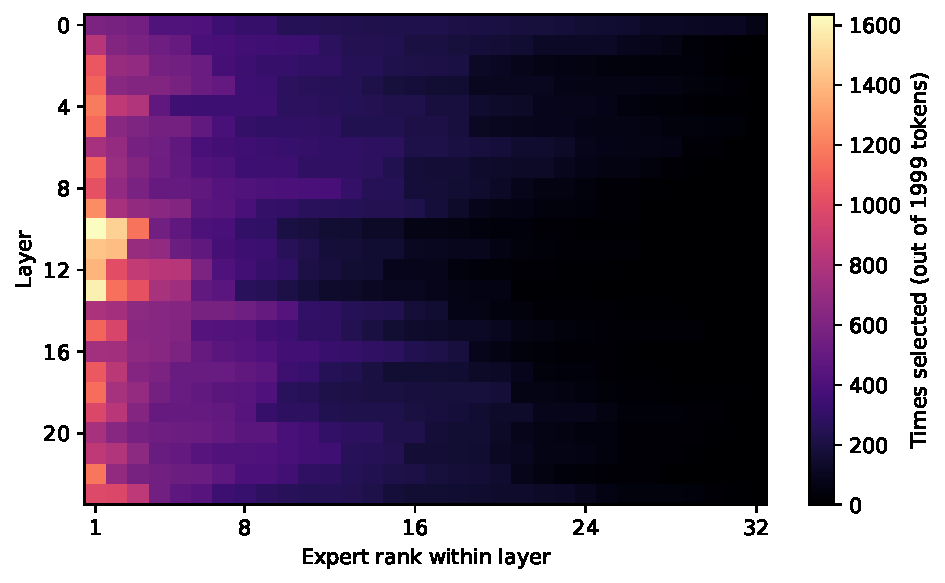
\includegraphics[width=0.85\textwidth]{figures/canon/expert_selection_heatmap.pdf}
\caption[Per-layer expert selection counts]{Selection counts for each (layer, expert) pair across 1999 generated tokens. Within each layer (row), the 32 experts are sorted by selection count descending, so column 1 is the layer's most-selected expert. Layers 10 to 13 fall off steeply (a few experts dominate the rest); layer 0 is much flatter.}
\label{fig:expert-selection-heatmap}
\end{figure}

The temporal access pattern is sharply skewed toward immediate reuse: 45.31\% of (layer, expert) reuses happen at the very next token, 76.14\% within five tokens, and 87.12\% within ten (\autoref{fig:reuse-distance-cdf}).
This is what makes a small in-memory cache effective even when its slot count sits below the per-token working set of 288: the experts that are about to be needed again are usually the ones just used.

\begin{figure}[htbp]
\centering
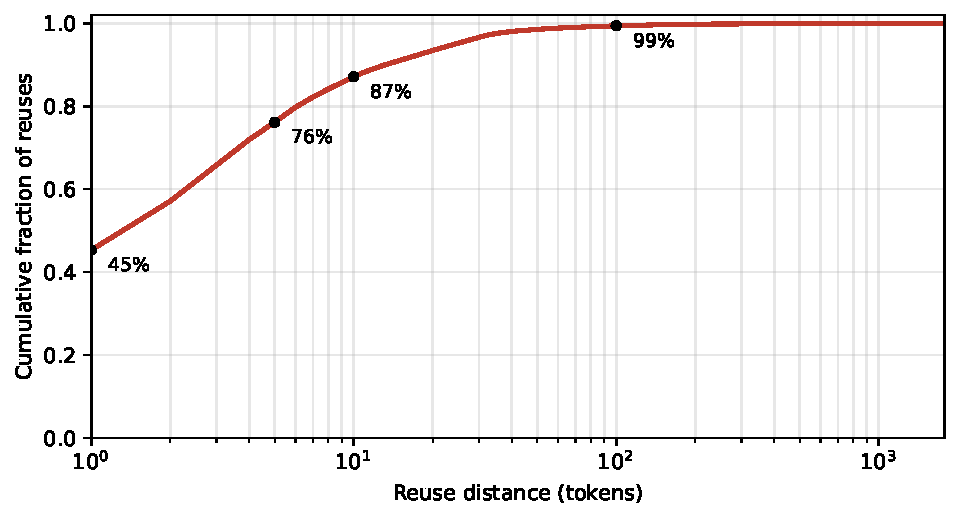
\includegraphics[width=0.85\textwidth]{figures/canon/reuse_distance_cdf.pdf}
\caption[Reuse-distance CDF for (layer, expert) selections]{Reuse distance for (layer, expert) selections in the canonical 1999-token decode. Distance is the number of tokens between two consecutive selections of the same (layer, expert) pair.}
\label{fig:reuse-distance-cdf}
\end{figure}


\section{Visualization}\label{sec:tracer-viz}

Two visualizers consume the per-token JSON.
The first is a browser-based viewer for one or two tokens at a time, with three synchronized views: a per-operation timeline, that token's computation graph, and a heatmap of reads against file offset.
The second is a native desktop application that drops the graph view in exchange for handling a hundred tokens or more, used for analysis across many tokens.


\section{Simulating Replacement}\label{sec:tracer-sim}

The simulator replays the buffer-access dump under five replacement policies and reports the resulting hit rate at a chosen cache size.
We compare LRU, LFU, LFU with periodic counter decay (LFU-aging), Adaptive Replacement Cache (ARC)~\cite{megiddo2003arc}, and W-TinyLFU~\cite{einziger2017tinylfu}.

\begin{table}[htbp]
\centering
\caption[Cache hit rate by policy and cache size]{Cache hit rate by replacement policy and cache size on the canonical 20B trace (1999 tokens, 575{,}724 expert weight accesses). The per-token working set is 288 slices. Bold marks the best policy at each cache size.}
\label{tab:tracer-policy-hits}
\begin{tabular}{lrrrrr}
\toprule
Cache slots & LRU & LFU & LFU-aging & ARC & W-TinyLFU \\
\midrule
200  &  0.00\% & 13.36\% & \textbf{29.08\%} &  0.00\% & 25.21\% \\
250  &  0.00\% & 16.85\% & \textbf{34.13\%} &  0.00\% & 31.05\% \\
288  & \textbf{36.02\%} & 19.47\% & 30.48\% & 32.92\% & 33.33\% \\
400  & 46.31\% & 28.97\% & 46.11\% & \textbf{48.04\%} & 42.39\% \\
500  & 54.88\% & 33.70\% & 54.03\% & \textbf{56.32\%} & 50.30\% \\
750  & 73.32\% & 46.77\% & 68.47\% & \textbf{73.68\%} & 70.40\% \\
1000 & 85.36\% & 62.02\% & 79.83\% & \textbf{85.46\%} & 77.46\% \\
\bottomrule
\end{tabular}
\end{table}

\begin{figure}[htbp]
\centering
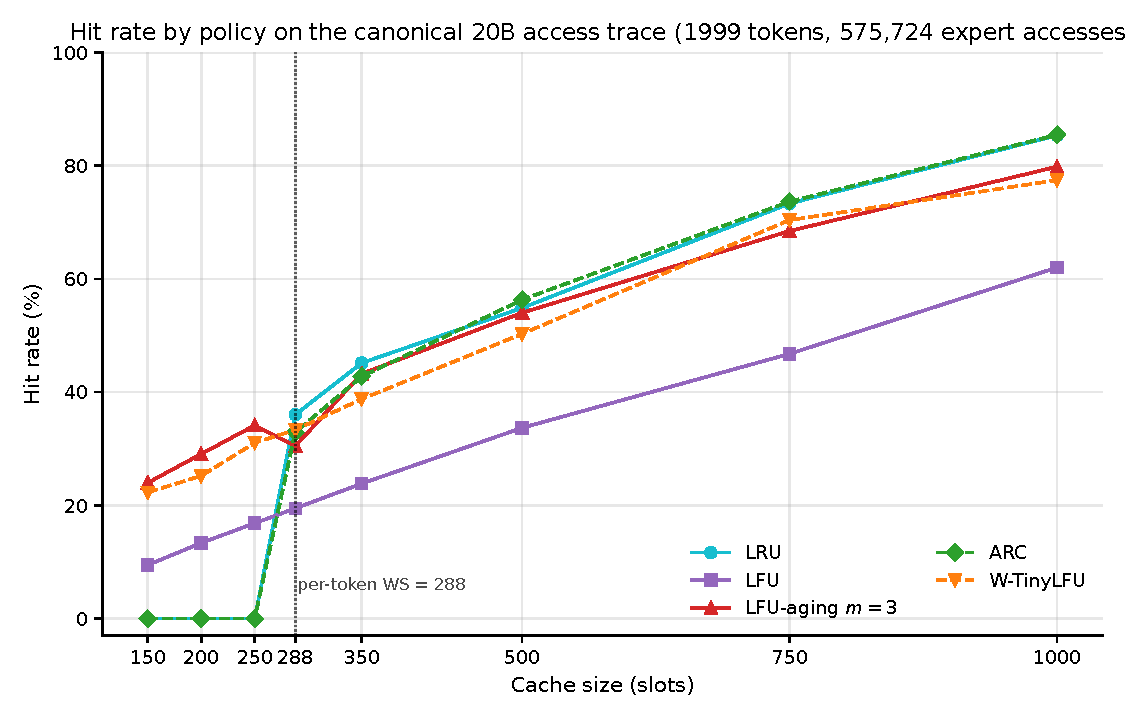
\includegraphics[width=0.85\textwidth]{figures/canon/lfu_lru_crossover.pdf}
\caption[Simulator hit rate by policy across cache sizes]{Simulator hit-rate curves on the canonical 20B trace, sweeping cache sizes from 150 to 1000 slots. The dotted vertical line marks the per-token working set of 288 slices, where the regime crossover happens: below it, LRU and ARC drop to zero while LFU-aging dominates; above it, LRU and ARC recover and lead.}
\label{fig:lfu-lru-crossover}
\end{figure}

The cache size relative to the per-token working set of 288 slices determines which policy wins.
Below the working set (200 and 250 slots), LRU and ARC produce zero hits: by the time a slice is selected for the second time, LRU has already evicted it, because the recency tail is exactly what is needed next.
LFU-aging dominates this regime by holding on to the small set of frequently-routed-to experts.
At and above the working set, LRU recovers, because the cache fits a token's reads with room to spare and per-access recency tracking now captures the immediate reuses of \autoref{fig:reuse-distance-cdf}.
LFU's counters suffer from stale popularity: experts that were heavily selected earlier in the run hold on to their slots after they have cooled.
ARC tracks LRU within a percentage point at every cache size where it is non-zero, and W-TinyLFU sits between the two extremes.

The simulator's LFU-aging implementation reproduces the hit rate of the deployed C runtime to within rounding (34.13\% simulated, 33.80\% measured at the canonical 7~GiB / 250-slot configuration), so the rankings in \autoref{tab:tracer-policy-hits} reflect what the runtime would observe.
The aging period was tuned on the simulator: counters are halved every $3 \times \mathit{cache\_slots}$ accesses, the highest-hit-rate multiplier we tested.
Routing-aware prefetching, which predicts the next layer's experts so their slices can be read ahead of time, is an active research direction~\cite{jia2025activeflow,xue2024moeinfinity} and is out of scope here.

\chapter{Implementation}\label{chapter:implementation}

\section{Pinning the dense weights}\label{sec:pinning}

The non-expert weights of the model file stay in the kernel-managed mmap region, and we mlock that region so the kernel cannot evict any of them.
The mlock excludes the experts (managed by the buffer of \autoref{sec:expert-buffer}) and the input embedding (each generated token reads only one of its rows).
Attention, the output projection, the layer norms, and the per-layer routers are therefore guaranteed resident throughout decode.


\section{The expert buffer}\label{sec:expert-buffer}

We replace the kernel's page-fault path for expert weights with \texttt{io\_uring}~\cite{axboe2019iouring} reads against an \texttt{O\_DIRECT}~\cite{open_man} file descriptor (\autoref{sec:bg-iouring}).
The application writes read requests into a shared submission ring, the kernel performs them in the background, and \texttt{O\_DIRECT} keeps the data out of the page cache so it transfers directly from the device into application buffers.
Together they let us submit many disk reads at once and pick up completions when convenient, with no intermediate copy in the page cache.

\texttt{O\_DIRECT} requires every read offset, length, and destination buffer address to be a multiple of 512 bytes.
The expert weight tensors in a GGUF file do not satisfy this.
We address the alignment with a one-time tool that reads every expert weight slice out of the GGUF and writes it into a sidecar file (\texttt{.bscexp}) at a 512-byte-aligned offset.
The sidecar is opened once per process with \texttt{O\_DIRECT}, and every \texttt{io\_uring} read targets a sidecar offset that is aligned by construction.

The buffer is a single 512-aligned anonymous region holding $N$ slots of 4.20~MiB each, where $N$ is configurable.
A hash map keyed by $(\mathit{layer}, \mathit{projection}, \mathit{expert\_id})$ returns the slot index of any resident slice.
On a hit, the buffer returns the slot's address.
On a miss, it picks a victim slot under the active replacement policy, issues a single \texttt{io\_uring} read into that slot, and returns the slot's address once the completion arrives.

Three replacement policies are implemented: LRU, LFU, and LFU-aging (the policies the simulator selected in \autoref{sec:tracer-sim}).
LRU keeps a doubly-linked list and promotes the slot on every access.
On a miss, the list's tail is evicted.
LFU and LFU-aging keep per-slot frequency counters and evict the slot with the smallest counter, with LFU-aging additionally halving every counter once per $3 \times \mathit{cache\_slots}$ accesses to discount stale popularity.
A per-load epoch prevents two misses in the same load from picking the same victim slot.


\section{Connecting the buffer to compute}\label{sec:buffer-integration}

The buffer's slices live in our own region of memory, separate from the mmap'd region of the model file that GGML's matrix-multiplication code normally reads from.
To make the slices visible to compute without copying, we use an existing GGML field: every tensor carries an opaque \texttt{extra} pointer that any computation in GGML can read freely.
Before each MoE layer runs, we fill \texttt{extra} with our array of slot pointers (one per active expert), and we patch the MoE matrix-multiplication function so that when \texttt{extra} is set, each active expert's address is taken from the array instead of from the tensor's base.
When \texttt{extra} is unset, the original code runs and no other operation in the model is affected.


\section{Pipelining I/O with compute}\label{sec:pipelining}

The simplest mode of the buffer is fully synchronous: a pre-compute callback before each layer submits all 12 reads as one \texttt{io\_uring} batch and waits for every completion before compute begins.
The three modes below progressively overlap I/O with compute, and each produces the same output as the synchronous path at fixed seed.


\subsection{Projection-group overlap}\label{sec:pipelining-po}

The down matmul takes the SwiGLU output as input, which means the down weights are not needed until SwiGLU has finished.
They can be loaded in the background while up, gate, and SwiGLU run.

We split the buffer's load into two phases inside a single callback before the up matmul.
Phase 1 submits the 8 up+gate reads as one \texttt{io\_uring} batch and waits for every completion.
Phase 2 submits the 4 down reads as a separate batch and returns immediately.
While the worker threads run up, gate, and SwiGLU on the up+gate slices, the 4 down reads complete in the background.
A second callback attached to the down matmul waits for any remaining down completions before down runs.

The 4 experts are still processed in a fixed order: each MoE matmul iterates them as $0, 1, 2, 3$ in turn (the positions in which the router emitted them).
Only the I/O is split.
The two phases share a single load epoch, which guarantees that phase 1's slots cannot be picked as eviction victims by phase 2.


\subsection{The fused MoE op}\label{sec:pipelining-fused}

In default llama.cpp, one MoE layer's feed-forward is a chain of separate GGML nodes: matmuls for up, gate, and down, plus SwiGLU and a per-expert accumulation.
Each matmul iterates the 4 selected experts internally.
The worker pool synchronizes at every node boundary, so all 4 experts finish their up matmul before any starts gate, and so on.
The structure is per-operation outside, per-expert inside.

Projection-group overlap fits this layout, because its callbacks attach to the existing nodes.
What the layout does not allow is starting one expert's down matmul while another expert is still loading from disk.
That would require inverting the loop nesting to per-expert outside, per-operation inside, and the per-node barriers prevent it.

We replace all of those default nodes with one fused custom GGML op.
From GGML's perspective, the entire MoE feed-forward is now one node, so GGML imposes no barrier inside it.
Inside, thread 0 picks the next compute action and issues any \texttt{io\_uring} submissions or waits the action requires.
All threads cross a barrier and cooperate on the picked action.
One barrier per dispatch round is enough, and the granularity at which we interleave I/O and compute is now ours to choose.

\begin{figure}[htbp]
\centering
\resizebox{0.95\textwidth}{!}{% Figure: GGML graph transformation for the fused MoE op.
% Compares the default graph (5 separate nodes) with our fused op (one node).
%
% Default (left): each MoE FFN layer is a chain of 5 GGML nodes. Each matmul
% node internally iterates over the 4 selected experts, and the worker pool
% synchronizes at every node boundary, so every expert finishes the current
% operation before any starts the next.
%
% Fused (right): the same compute is collapsed into one custom GGML node.
% Inside the node, our own dispatch loop runs the io_uring submissions, picks
% the next compute action under a state machine, and synchronizes the worker
% pool with an atomic barrier of our own.

\begin{tikzpicture}[
  font=\footnotesize,
  default_node/.style={
    draw=TUMSecondaryBlue!70!black, fill=TUMSecondaryBlue!12,
    rounded corners=2pt,
    minimum width=28mm, minimum height=7mm,
    align=center
  },
  fused_outer/.style={
    draw=TUMAccentGreen!75!black, fill=TUMAccentGreen!5,
    line width=0.8pt, rounded corners=4pt,
    minimum width=44mm, minimum height=46mm
  },
  fused_inner/.style={
    draw=TUMAccentGreen!60!black, fill=TUMAccentGreen!18,
    rounded corners=2pt,
    minimum width=36mm, minimum height=7mm,
    align=center, font=\scriptsize
  },
  arr/.style={->, line width=0.45pt, draw=black!75},
  hdr/.style={font=\sffamily\bfseries\small, align=center},
  foot/.style={font=\scriptsize, text=black!65, align=center},
]

  % --- LEFT column: default graph ---
  \node[hdr] at (0, 7.0) {Default GGML graph};

  \node[default_node] (up_d)     at (0, 5.5) {matmul (up)};
  \node[default_node] (gate_d)   at (0, 4.4) {matmul (gate)};
  \node[default_node] (swiglu_d) at (0, 3.3) {SwiGLU};
  \node[default_node] (down_d)   at (0, 2.2) {matmul (down)};
  \node[default_node] (acc_d)    at (0, 1.1) {accumulate};

  \draw[arr] (up_d)     -- (gate_d);
  \draw[arr] (gate_d)   -- (swiglu_d);
  \draw[arr] (swiglu_d) -- (down_d);
  \draw[arr] (down_d)   -- (acc_d);

  \node[foot] at (0, 0.0)
    {each matmul iterates 4 experts internally.\\Worker pool synchronizes at every node boundary.};

  % --- middle: replacement arrow ---
  \node[font=\Large] at (5.6, 3.3) {$\Rightarrow$};

  % --- RIGHT column: fused op ---
  \node[hdr] at (9.0, 7.0) {Fused custom GGML op};

  \node[fused_outer] (fused) at (9.0, 3.3) {};

  \node[fused_inner] (sm)      at (9.0, 5.0) {state-machine picker};
  \node[fused_inner] (iouring) at (9.0, 4.0) {\texttt{io\_uring} submit / wait};
  \node[fused_inner] (compute) at (9.0, 3.0) {up, gate, SwiGLU, down};
  \node[fused_inner] (acc_f)   at (9.0, 2.0) {accumulate};

  \draw[arr] (sm)      -- (iouring);
  \draw[arr] (iouring) -- (compute);
  \draw[arr] (compute) -- (acc_f);

  \node[foot] at (9.0, 0.0)
    {one node from GGML's view.\\Internal dispatch under our control.};

\end{tikzpicture}
}
\caption[Default GGML graph versus the fused MoE op]{Default GGML graph (left) versus the fused custom op (right). The 5 separate nodes on the left are subject to GGML's per-node barriers, which fix the loop nesting to per-operation outside, per-expert inside. Collapsing them into one node on the right places the dispatch loop inside our control, so the per-expert and per-matmul dispatch in the next two subsections become possible.}
\label{fig:moe-fused-op}
\end{figure}


\subsection{Async-projection-overlap}\label{sec:pipelining-apo}

Async-projection-overlap differs from projection-group overlap in two ways.
All 12 reads are submitted at the start of the fused op, not split into two phases.
The 4 experts are processed in the order their data arrives, not in $0, 1, 2, 3$ position order.

Each expert's up and gate reads share one \texttt{io\_uring} tag and its down read takes a separate tag, for $4 \times 2 = 8$ tags in flight together.
Thread 0 waits for any one of the 4 up+gate pairs to complete and dispatches that expert.
The worker threads run up, gate, and SwiGLU on that expert.
Thread 0 then waits for that expert's down read (in flight since layer entry) before the worker threads run down.
Thread 0 picks the next first-ready expert from the remaining tags and the loop repeats until all 4 have run.

Each expert's output is written into a slot at its router-assigned position, and the 4 slots are summed in position order at the end of the op, so the final output matches the synchronous and projection-group overlap paths.


\subsection{Async-experts}\label{sec:pipelining-ae}

Async-experts pushes the dispatch granularity one step finer.
Where async-projection-overlap dispatches per expert (each expert runs up + gate + SwiGLU + down end-to-end before the next expert starts), async-experts dispatches per individual matmul: an expert's up matmul can run as soon as its up tag completes, even before its gate read has arrived.

Each projection of each expert gets its own \texttt{io\_uring} tag, for $4 \times 3 = 12$ tags in flight together.
Thread 0 maintains a per-expert state machine and at each dispatch round walks the 4 active experts in order, picking the first eligible action (\autoref{fig:async-experts-state}).
When the second of an expert's two pre-SwiGLU matmuls completes, SwiGLU and the down-input quantization fold into the same dispatch round, so SwiGLU is never a standalone action.

\begin{figure}[htbp]
\centering
\resizebox{0.85\textwidth}{!}{% Figure: per-expert state machine for the async-experts dispatcher.
% Matches the actual implementation in llama-moe-pipeline.cpp:
%   AE_UP_MATMUL        : up only (gate not yet computed)
%   AE_UP_AND_FINISH    : up + swiglu + quantize (gate already computed)
%   AE_GATE_MATMUL      : gate only (up not yet computed)
%   AE_GATE_AND_FINISH  : gate + swiglu + quantize (up already computed)
%   AE_DOWN_MATMUL      : down only
%
% The fold-in optimization (AND_FINISH variants) collapses SwiGLU and the
% down-input quantize into the second-arrival matmul, so there is no
% standalone "both matmuls done, no swiglu" intermediate state.
%
% Conventions:
%   * S_0 (green)  : initial, nothing computed
%   * S_1          : up matmul done first
%   * S_2          : gate matmul done first
%   * S_3          : SwiGLU + quantize done; ready for down
%   * S_4 (orange) : down matmul done; expert complete
%   * Edge labels  : action above (blue), io_uring completion guard below
%                    (italic orange)

\begin{tikzpicture}[
    font=\sffamily\small,
    >={Latex[length=2.5mm]},
    state/.style={
        draw, rounded corners=2pt, fill=TUMLightGray!20,
        minimum width=18mm, minimum height=11mm, align=center,
        inner sep=2pt,
        font=\sffamily\small,
    },
    initstate/.style={state, fill=TUMAccentGreen!20, draw=TUMAccentGreen!60!black},
    finalstate/.style={state, fill=TUMAccentOrange!25, draw=TUMAccentOrange!70!black},
    actlabel/.style={font=\scriptsize\sffamily, text=TUMSecondaryBlue, inner sep=1.5pt},
    guardlabel/.style={font=\scriptsize\sffamily\itshape, text=TUMAccentOrange!85!black, inner sep=1.5pt},
]
  % --- States ---
  \node[initstate]  (s0) at (0,    0)    {$S_0$\\[1pt]\scriptsize init};
  \node[state]      (s1) at (4.5,  1.6)  {$S_1$\\[1pt]\scriptsize up done};
  \node[state]      (s2) at (4.5, -1.6)  {$S_2$\\[1pt]\scriptsize gate done};
  \node[state]      (s3) at (9.0,  0)    {$S_3$\\[1pt]\scriptsize SwiGLU done};
  \node[finalstate] (s4) at (13.5, 0)    {$S_4$\\[1pt]\scriptsize complete};

  % --- S_0 to first-arrival branches (diamond top + bottom) ---
  \draw[->, thick] (s0) -- (s1)
      node[actlabel,   sloped, above, pos=0.5] {up matmul}
      node[guardlabel, sloped, below, pos=0.5] {loaded\_up};
  \draw[->, thick] (s0) -- (s2)
      node[actlabel,   sloped, above, pos=0.5] {gate matmul}
      node[guardlabel, sloped, below, pos=0.5] {loaded\_gate};

  % --- Second-arrival fold-in: AND_FINISH variants merge to S_3 ---
  \draw[->, thick] (s1) -- (s3)
      node[actlabel,   sloped, above, pos=0.5, align=center] {gate matmul\\+ SwiGLU + quant}
      node[guardlabel, sloped, below, pos=0.5] {loaded\_gate};
  \draw[->, thick] (s2) -- (s3)
      node[actlabel,   sloped, above, pos=0.5, align=center] {up matmul\\+ SwiGLU + quant}
      node[guardlabel, sloped, below, pos=0.5] {loaded\_up};

  % --- Final transition to S_4 ---
  \draw[->, thick] (s3) -- (s4)
      node[actlabel,   above, pos=0.5] {down matmul}
      node[guardlabel, below, pos=0.5] {loaded\_down};
\end{tikzpicture}
}
\caption[Per-expert state machine for async-experts]{Per-expert state machine inside the async-experts dispatch loop. $S_0$ is the initial state. The diamond $S_0 \to \{S_1, S_2\} \to S_3$ captures the difference from async-projection-overlap: an expert's first matmul runs as soon as one of its up or gate reads completes, without waiting for the other. The second-arrival matmul folds SwiGLU and the down-input quantization into the same dispatch round (the \emph{and finish} variants), so $S_3$ is the post-SwiGLU state ready for the down matmul.}
\label{fig:async-experts-state}
\end{figure}

The same position-order summation at the end makes the output identical to async-projection-overlap.
In our wall-clock measurements (\autoref{chapter:evaluation}), async-experts lands within roughly one percent of async-projection-overlap, so we keep async-projection-overlap as the deployed configuration.


\chapter{Evaluation}\label{chapter:evaluation}

This chapter measures our backend against the default llama.cpp loader on the same hardware under a kernel-enforced RAM limit.


\section{Setup}\label{sec:eval-setup}\label{sec:eval-hardware}

The test machine runs Linux on an AMD Ryzen 7 7700X (8 cores) with 30~GiB of DDR5 main memory and two NVMe SSDs~\cite{amd_ryzen7700x,jedec_ddr5}.
The operating system lives on the first SSD.
The second is a 1~TB Samsung 980~PRO over PCIe~4.0~\cite{pcisig_pcie4} dedicated to the model files and their sidecar pack files (\autoref{sec:expert-buffer}); all reported numbers come from this drive, so model I/O is not mixed with operating-system activity during measurement.

We control RAM by launching the inference process inside a transient systemd scope under cgroup~v2 with \texttt{memory.max} set to the limit we want and \texttt{MemorySwapMax=0}, with system swap also disabled~\cite{cgroupv2}.
An allocation that would push the process over the cgroup limit fails immediately rather than spilling to disk.
Each measurement runs 2000 tokens of decode at seed 42 from a multi-topic prompt, kernel page caches are dropped before every run, and the reported throughput is decode token count divided by decode time.
All measurements use the \texttt{--eager-compute} flag, which forces the compute buffer resident at graph reservation so the cgroup count is deterministic.

The cgroup limit covers everything the inference process holds.
A fixed footprint goes to the pinned dense weights (\autoref{sec:pinning}), the KV cache, the compute buffer, and a small amount of miscellaneous anonymous memory.
The remainder, less a safety margin, holds our expert buffer (\autoref{sec:expert-buffer}) at 4.20~MiB per slot.
\autoref{tab:eval-fixed-footprint} lists the breakdown for both models.

\begin{table}[htbp]
\centering
\caption[Fixed memory footprint per model]{Fixed memory footprint of the inference process under the cgroup limit. The remainder of the limit, less a safety margin, holds the expert buffer at 4.20~MiB per slot.}
\label{tab:eval-fixed-footprint}
\begin{tabular}{lrr}
\toprule
Component & GPT-OSS-20B & GPT-OSS-120B \\
\midrule
Pinned dense weights         & 2.27~GiB & 2.98~GiB \\
KV cache (\texttt{ctx=131072}) & 3.02~GiB & 4.53~GiB \\
Compute buffer (eager)       & 0.40~GiB & 0.40~GiB \\
Misc anonymous               & 0.18~GiB & 0.23~GiB \\
\midrule
Fixed footprint (sum)        & 5.87~GiB & 8.14~GiB \\
\bottomrule
\end{tabular}
\end{table}

For each cgroup limit, the cache slot count is sized to fill the remaining space: 250 / 498 / 740 slots at 7 / 8 / 9~GiB on GPT-OSS-20B, and 693 / 1668 / 3130 / 4592 slots at 12 / 16 / 22 / 28~GiB on GPT-OSS-120B.
Across the 168 runs of the canonical sweep (56 cells $\times$ 3 iterations across both models), the mean coefficient of variation in decode time is 0.23\%.


\section{GPT-OSS-20B}\label{sec:eval-20b}

\autoref{tab:eval-20b-headline} reports decode throughput on GPT-OSS-20B (12.85~GiB on disk) at four cgroup limits.
At the smallest three cells (7, 8, 9~GiB), the working set exceeds the available RAM once the pinned weights, KV cache, and compute buffer are accounted for, so the model file's pages have to turn over every layer.
The 22~GiB cell leaves enough RAM for the model to stay fully resident.

% Auto-generated by thesis/scripts/tables_canon.py from _meta/final_canon.json.
% Do not hand-edit. Re-run the script if the oracle changes.

\begin{table}[htbp]
\centering
\caption[GPT-OSS-20B throughput at four cgroup budgets]{GPT-OSS-20B throughput at four cgroup limits, three iterations per cell. Each block is monotonic top to bottom when the model does not fit in RAM: pinning helps in proportion to what the kernel would otherwise evict, and our buffer-managed I/O stack adds roughly an additional $2\times$ on top. At 22~GiB the working set fits and all configurations converge.}
\label{tab:eval-20b-headline}
\begin{tabular}{lrrr}
\toprule
Configuration & Tok/s & Eval CV (\%) & Speedup vs lazy \\
  \midrule
  \multicolumn{4}{l}{\textit{cgroup memory.max = 7~GiB}} \\
  lazy mmap                      & 1.44 & 0.15 & 1.00$\times$ \\
  mmap $+$ pin                   & 2.24 & 0.76 & 1.55$\times$ \\
  \multicolumn{4}{l}{\textit{with buffer: 250 slots ($\approx$ 1.03~GiB), $\approx$ 0.10~GiB free}} \\
  projection-group overlap       & 5.02 & 0.32 & 3.49$\times$ \\
  async-projection-overlap       & \textbf{5.36} & 0.48 & 3.72$\times$ \\
  async-experts                  & 5.11 & 1.63 & 3.55$\times$ \\
  \midrule
  \multicolumn{4}{l}{\textit{cgroup memory.max = 8~GiB}} \\
  lazy mmap                      & 2.67 & 0.04 & 1.00$\times$ \\
  mmap $+$ pin                   & 3.50 & 0.17 & 1.31$\times$ \\
  \multicolumn{4}{l}{\textit{with buffer: 498 slots ($\approx$ 2.04~GiB), $\approx$ 0.08~GiB free}} \\
  projection-group overlap       & 6.18 & 0.09 & 2.31$\times$ \\
  async-projection-overlap       & 6.52 & 0.18 & 2.44$\times$ \\
  async-experts                  & \textbf{6.59} & 2.29 & 2.47$\times$ \\
  \midrule
  \multicolumn{4}{l}{\textit{cgroup memory.max = 9~GiB}} \\
  lazy mmap                      & 3.86 & 0.08 & 1.00$\times$ \\
  mmap $+$ pin                   & 4.68 & 0.12 & 1.21$\times$ \\
  \multicolumn{4}{l}{\textit{with buffer: 740 slots ($\approx$ 3.04~GiB), $\approx$ 0.09~GiB free}} \\
  projection-group overlap       & 8.14 & 0.01 & 2.11$\times$ \\
  async-projection-overlap       & \textbf{8.70} & 0.03 & 2.25$\times$ \\
  async-experts                  & 8.57 & 0.01 & 2.22$\times$ \\
  \midrule
  \multicolumn{4}{l}{\textit{cgroup memory.max = 22~GiB; model fits in RAM}} \\
  lazy mmap                      & \textbf{14.32} & 0.04 & 1.00$\times$ \\
  mmap $+$ pin                   & 14.29 & 0.06 & 1.00$\times$ \\
  projection-group overlap       & 14.04 & 0.06 & 0.98$\times$ \\
  async-projection-overlap       & 13.92 & 0.02 & 0.97$\times$ \\
  async-experts                  & 13.90 & 0.11 & 0.97$\times$ \\
\bottomrule
\end{tabular}
\end{table}

\begin{table}[htbp]
\centering
\caption[GPT-OSS-120B throughput at four cgroup budgets]{GPT-OSS-120B throughput at four cgroup limits, three iterations per cell. GPT-OSS-120B (60.88~GiB on disk) exceeds the host's 30~GiB RAM by a factor of about 2, so every cell forces page-cache turnover regardless of the cgroup limit. The configuration ranking is the same as on the smaller model, and our buffer-managed I/O stack adds a factor of roughly $1.63$--$2.38\times$ on top of pin.}
\label{tab:eval-120b-headline}
\begin{tabular}{lrrr}
\toprule
Configuration & Tok/s & Eval CV (\%) & Speedup vs lazy \\
  \midrule
  \multicolumn{4}{l}{\textit{cgroup memory.max = 12~GiB}} \\
  lazy mmap                      & 1.50 & 0.10 & 1.00$\times$ \\
  mmap $+$ pin                   & 1.89 & 0.21 & 1.26$\times$ \\
  \multicolumn{4}{l}{\textit{with buffer: 693 slots ($\approx$ 2.84~GiB), $\approx$ 1.02~GiB free}} \\
  projection-group overlap       & 3.37 & 0.09 & 2.25$\times$ \\
  async-projection-overlap       & \textbf{3.58} & 0.02 & 2.38$\times$ \\
  async-experts                  & 3.54 & 0.03 & 2.36$\times$ \\
  \midrule
  \multicolumn{4}{l}{\textit{cgroup memory.max = 16~GiB}} \\
  lazy mmap                      & 2.25 & 0.15 & 1.00$\times$ \\
  mmap $+$ pin                   & 2.55 & 0.16 & 1.13$\times$ \\
  \multicolumn{4}{l}{\textit{with buffer: 1668 slots ($\approx$ 6.84~GiB), $\approx$ 1.02~GiB free}} \\
  projection-group overlap       & 4.55 & 0.23 & 2.02$\times$ \\
  async-projection-overlap       & \textbf{4.89} & 0.02 & 2.17$\times$ \\
  async-experts                  & 4.81 & 0.16 & 2.13$\times$ \\
  \midrule
  \multicolumn{4}{l}{\textit{cgroup memory.max = 22~GiB}} \\
  lazy mmap                      & 3.50 & 0.12 & 1.00$\times$ \\
  mmap $+$ pin                   & 3.72 & 0.10 & 1.07$\times$ \\
  \multicolumn{4}{l}{\textit{with buffer: 3130 slots ($\approx$ 12.84~GiB), $\approx$ 1.03~GiB free}} \\
  projection-group overlap       & 6.23 & 0.25 & 1.78$\times$ \\
  async-projection-overlap       & \textbf{6.66} & 0.02 & 1.90$\times$ \\
  async-experts                  & 6.57 & 0.05 & 1.88$\times$ \\
  \midrule
  \multicolumn{4}{l}{\textit{cgroup memory.max = 28~GiB}} \\
  lazy mmap                      & 4.96 & 0.33 & 1.00$\times$ \\
  mmap $+$ pin                   & 5.17 & 0.18 & 1.04$\times$ \\
  \multicolumn{4}{l}{\textit{with buffer: 4592 slots ($\approx$ 18.83~GiB), $\approx$ 1.03~GiB free}} \\
  projection-group overlap       & 7.70 & 0.30 & 1.55$\times$ \\
  async-projection-overlap       & \textbf{8.06} & 0.04 & 1.63$\times$ \\
  async-experts                  & 7.99 & 0.01 & 1.61$\times$ \\
\bottomrule
\end{tabular}
\end{table}

\begin{table}[htbp]
\centering
\caption[Cache eviction policy at 20B 7~GiB c=250]{Cache eviction policy comparison at GPT-OSS-20B, cgroup memory.max~=~7~GiB, cache 250 slots (below the per-token working set of 288). Three iterations per cell, all CVs $\leq$~1.7\%. All values in tokens per second. LFU-aging dominates LFU dominates LRU at every io\_uring code path: when the cache is below the working set, the LRU tail is exactly the next slice the access pattern asks for and the policy thrashes.}
\label{tab:cache-policy-7g}
\begin{tabular}{lrrr}
\toprule
io\_uring code path & LRU & LFU & LFU-aging $m=3$ \\
\midrule
  uring (sync)                   & 3.65 & 4.15 & \textbf{4.82} \\
  projection-group overlap       & 3.80 & 4.31 & \textbf{5.02} \\
  async-projection-overlap       & 3.98 & 4.58 & \textbf{5.36} \\
  async-experts                  & 3.87 & 4.38 & \textbf{5.11} \\
\bottomrule
\end{tabular}
\end{table}

\begin{table}[htbp]
\centering
\caption[Reproducibility of the May 1/2 canonical sweep]{Reproducibility of the May 1/2 canonical sweep across all 56 configurations and 168 total iterations. Mean coefficient of variation in eval seconds is 0.23\%; median 0.101\%; max 2.29\%. The kernel-enforced cgroup memory.max methodology is reproducible at the sub-percent level on this hardware.}
\label{tab:reproducibility}
\begin{tabular}{lr}
\toprule
Statistic & Value \\
\midrule
Configurations    & 56 \\
Iterations / cell & 3 \\
Total runs        & 168 \\
Mean CV (\%)      & 0.23 \\
Median CV (\%)    & 0.101 \\
Max CV (\%)       & 2.29 \\
Configs with CV $<$ 0.5\% & 49 of 56 \\
\bottomrule
\end{tabular}
\end{table}


The configuration order is monotonic at the three smaller cells.
Pinning the dense weights (\autoref{sec:pinning}) helps in proportion to what the kernel would otherwise evict: $1.55\times$ over lazy mmap at 7~GiB, $1.21\times$ at 9~GiB.
Replacing the synchronous fault path with our buffer plus projection-group overlap (\autoref{sec:pipelining-po}) adds the largest single jump, roughly a further factor of two over pin.
Async-projection-overlap (\autoref{sec:pipelining-apo}) reaches 5.36 / 6.52 / 8.70~tok/s at 7 / 8 / 9~GiB ($3.72\times$, $2.44\times$, and $2.25\times$ over the lazy mmap baseline) and is the fastest configuration at 7 and 9~GiB.
At 8~GiB async-experts (\autoref{sec:pipelining-ae}) edges it at 6.59~tok/s, by an amount that sits inside the run-to-run noise of that cell (\autoref{sec:eval-overlap}).

The 22~GiB cell is the upper bound on this hardware for this model.
With the working set entirely resident, the kernel page cache holds every weight, the synchronous fault path stops being a cost we have to remove, and all five configurations converge to within 0.42~tok/s of each other at 13.90--14.32~tok/s.
Our backend in fact loses about 0.40~tok/s relative to plain mmap at this cell. The cache is sized to 2304 slots, exactly the full expert population ($24$~layers $\times$ $32$~experts $\times$ $3$~projections), so once it warms neither path makes runtime I/O and what remains is overhead in the buffer-managed code path that the I/O savings at smaller cells more than offset.
Every speedup the rest of this chapter reports is the speedup available when the RAM cap is tight. In its absence the buffer-managed I/O path is a small net cost.


\section{GPT-OSS-120B}\label{sec:eval-120b}

\autoref{tab:eval-120b-headline} reports the same sweep on GPT-OSS-120B (60.88~GiB on disk).
The model exceeds host RAM by a factor of about 2, so every cell forces page-cache turnover regardless of the cgroup limit; even at 28~GiB the page cache cannot hold the full set of expert weights.

The configuration order is the same as on the smaller model.
Pinning helps less in absolute terms (4--26\% over lazy mmap rather than 21--55\%) because the cgroup budgets here (12--28~GiB) leave the kernel page cache more headroom than the 2.98~GiB of dense weights need: even the 12~GiB cell has roughly 6.8~GiB free for the page cache, so the kernel's own LRU keeps most dense pages resident without help. Pinning's marginal value is what the kernel would otherwise evict, and at these budgets that is a small share of dense reads.
Async-projection-overlap is the fastest configuration at every cell, reaching 8.06~tok/s at 28~GiB against 4.96~tok/s for lazy mmap, a $1.63\times$ speedup.
There is no fully-resident cell here in our cgroup range: even at 28~GiB the model is more than twice the available RAM, so I/O dominates every run.


\section{Cache eviction policy at undersized cache}\label{sec:eval-policy}

The 7~GiB cell on GPT-OSS-20B fixes the buffer at 250 slots, which is below the 288-slice per-token working set established in \autoref{sec:tracer-sim}.
The simulator there predicts that LFU-aging dominates LFU dominates LRU when the cache holds fewer slots than the working set.
\autoref{tab:cache-policy-7g} confirms this at wall-clock time across all four io\_uring code paths.

At the headline async-projection-overlap cell, LFU-aging reaches 5.36~tok/s against LRU's 3.98~tok/s. The simulator's hit-rate prediction in \autoref{tab:tracer-policy-hits} explains the gap: LRU at 250 slots produces a 0.00\% hit rate, so every expert access pays a fresh disk read, while LFU-aging holds 34.13\%. The mechanism behind the zero (described in \autoref{sec:tracer-sim}) is that the cyclic per-token access pattern places LRU's tail on exactly the slice it is about to ask for next, so each new arrival evicts what is needed immediately afterward. Per-slot frequency counters protect the small set of frequently-routed-to experts and avoid that geometry.
At 8~GiB and 9~GiB the cache (498 / 740 slots) exceeds the working set and we use LRU, because each expert's three slices (up, gate, down) are read in immediate succession within a layer, which LRU's per-access promotion captures cleanly.
The same regime argument applies to every GPT-OSS-120B cell in our sweep, where the cache always holds more slots than the per-token working set.


\section{Comparing the overlap modes}\label{sec:eval-overlap}

The three pipelining modes that overlap I/O with compute (projection-group overlap, async-projection-overlap, async-experts) all produce the same output at fixed seed, so the comparison between them is purely wall-clock.

Across the seven cells where the model does not fit (GPT-OSS-20B at 7, 8, 9~GiB; GPT-OSS-120B at 12, 16, 22, 28~GiB), async-projection-overlap is the fastest at six of seven.
Projection-group overlap consistently lags it by 4.47 to 6.95\% (on GPT-OSS-20B at 9~GiB it is 8.14 vs 8.70~tok/s, a 6.44\% gap).
Async-experts lands within 1.49\% of async-projection-overlap at every cell, for example 8.57 vs 8.70~tok/s at GPT-OSS-20B 9~GiB and 7.99 vs 8.06~tok/s at GPT-OSS-120B 28~GiB.
The 20B 8~GiB cell is the only one where async-experts edges async-projection-overlap (6.59 vs 6.52~tok/s), by an amount inside the cell's run-to-run noise.

Async-projection-overlap is therefore the deployed configuration.
Async-experts is within noise of it on this hardware.
Projection-group overlap is a few percent behind because the down reads only have one compute window to hide behind, while the two async modes can overlap each expert's I/O with the compute of every preceding expert in the layer.

\chapter{Discussion and Conclusion}\label{chapter:closing}

\section{Limitations}\label{sec:limitations}

The headline numbers come from a single host running a multi-topic prompt at a fixed seed across both models.
Three caveats follow from that.

\begin{itemize}
\item The hardware is one consumer-class configuration: an 8-core AMD CPU, 30~GiB of DDR5, and a single PCIe~4.0 NVMe SSD as the model store.
A different CPU would shift the 22~GiB CPU-bound ceiling on GPT-OSS-20B.
A slower SSD would shrink the absolute speedups of the buffered modes.

\item Wall-clock numbers come from one prompt domain.
We separately captured tensor-level traces on five additional prompts (code, mathematical reasoning, creative writing, factual explanation, and a mixed code-plus-prose prompt).
The simulator's hit rate at the headline 250-slot LFU-aging configuration spans 32.6\% (mixed) to 43.0\% (creative), a 10.4 pp spread, and reuse-distance-1 spans 43--50\% across the same six domains.
Translating the hit-rate spread through our empirical hit-rate-to-tok/s sensitivity points to a few percent of cross-domain wall-clock variation, but we did not run end-to-end wall-clock measurements on the five extra domains.

\item Two replacement policies (ARC and W-TinyLFU) appear only in the simulator, not in the C runtime.
The simulator's predictions match the deployed policies to within rounding, but a live C implementation would close the loop in the operating regime where LRU and LFU-aging already perform within noise of each other.
\end{itemize}


\section{Future work}\label{sec:future-work}

Four directions extend naturally from where this thesis stops.

\paragraph{Cross-layer expert prefetching.}
The pipelining work in this thesis stops at the layer boundary, because the router's choice of next-layer experts is independent of the current layer's hidden state in any way we can predict cheaply.
A small router-prediction head, trained to forecast layer~$N{+}1$'s expert IDs from layer~$N$'s output, would let the loader start the disk reads one layer earlier and hide more of the I/O behind compute.
This is a separate research direction (expert speculation).

\paragraph{Request-similarity prefetch.}
The current system carries no state between requests.
Every request starts with an empty cache and pays the cold-start miss for each first-touch expert.
MoE-Infinity~\cite{xue2024moeinfinity} records each completed request as a small Expert Activation Matrix (rows are layers, columns are experts, entries are how often each expert was selected) and matches an in-flight request against historical ones by cosine similarity to drive prefetch.
The construction transfers cleanly to our setting: a few kilobytes per stored matrix, microsecond cosine matching, and a populated cache before the first decode token.
It targets a phase the per-token working-set arithmetic in \autoref{chapter:tracer} cannot address, and it is orthogonal to the router-prediction head above (cross-request fingerprint at request start versus cross-layer router prediction during decode).

\paragraph{Faster startup via lazy pinning.}
The current pinning mlocks the dense weight pages eagerly at model-load time.
Linux's \texttt{mlock2} with the \texttt{MLOCK\_ONFAULT} flag~\cite{mlock2_man} marks pages non-reclaimable but defers the actual residency until first fault.
For a generation-time workload this would shift the load-time cost into the first forward pass without changing steady-state behaviour.

\paragraph{GPU integration.}
The work in this thesis is entirely CPU-side.
The I/O architecture (the buffer manager, the sidecar pack file, the per-expert tagged completions) is orthogonal to the compute backend.
A GPU compute path would still need expert weights resident in some buffer before launch and the same routing-driven cache.
The integration question is the boundary: \texttt{O\_DIRECT} reads can target GPU-resident memory through GPUDirect Storage~\cite{nvidia_gds} or analogous facilities, pushing the buffer onto the device and keeping the CPU out of the data path.

\section{Conclusion}\label{sec:thesis-conclusion}

Modern open-source language models hold large amounts of weight data on disk.
The two studied here, GPT-OSS-20B and GPT-OSS-120B, weigh 12.85~GiB and 60.88~GiB respectively, against the 30~GiB of RAM on our test machine.
RAM is expensive, NVMe SSDs are not, and a Mixture-of-Experts model reads only a small fraction of its weights per generated token.

We built a tensor-level tracer to see what the model actually reads, and the trace showed a non-uniform access pattern: the dense per-layer weights are read on every token, while only a few experts per layer per token are selected by the router.
We pinned the dense weights in RAM so the kernel could not evict them, and we managed the experts ourselves in a buffer that reads from the SSD asynchronously, with three loading strategies of increasing aggressiveness.
The most aggressive submits all of a layer's expert reads at the start of the layer and dispatches each expert's compute as its data arrives.

With 7~GiB of RAM available, our backend lifts GPT-OSS-20B from 1.44~tok/s under the default loader to 5.36~tok/s, almost four times faster.
GPT-OSS-120B does not fit in our 30~GiB of RAM at all.
The default loader runs it at 4.96~tok/s and our backend at 8.06~tok/s.
A simulator built on the same trace lays a foundation for choosing the cache replacement policy and confirms the wall-clock observation that LFU-aging dominates when the cache is below the per-token working set, while LRU wins above it.

The tracer, the buffer-managed loader, the simulator, and the patched llama.cpp fork are released as artifacts (\autoref{chapter:artifacts}) so the path from question to answer can be walked again on different hardware, a different model, or a different storage stack.


\appendix{}

\chapter{Software Artifacts}\label{chapter:artifacts}

\paragraph{Prerequisites.} The reproduction recipes below assume a Linux 5.6+ kernel with cgroup~v2~\cite{cgroupv2} mounted at \texttt{/sys/fs/cgroup/}, \texttt{liburing} 2.0+ headers, GCC 11+, CMake 3.20+, and a user account with \texttt{sudo} for cgroup creation and kernel-cache drop operations. System swap must be disabled (\texttt{sudo swapoff -a}) so cgroup \texttt{MemorySwapMax=0} is enforceable end-to-end. The model file must be a GPT-OSS-20B or GPT-OSS-120B GGUF in F16 quantization~\cite{openai2025gptoss} from the \texttt{ggml-org/gpt-oss-*-GGUF} repositories on Hugging Face. The \texttt{.bscexp} sidecar is produced by the \texttt{bsc-pack-experts} preprocessor at first run (\autoref{sec:art-llamacpp}). The test machine described in \autoref{sec:eval-hardware} is the reference hardware; the methodology transfers to any host with NVMe-attached storage.


\section{Forked llama.cpp}\label{sec:art-llamacpp}

Repository: \texttt{github.com/ErsjanKeri/llama.cpp}, default branch \texttt{master}, tag \texttt{bsc-thesis-v1} (commit \texttt{5aec1115}). The fork carries twenty-six commits on top of upstream llama.cpp \cite{ggerganov2023llamacpp} covering the tensor tracer, the io\_uring + O\_DIRECT expert loader, the fused MoE custom op, and the three pipeline modes (projection-group overlap, async-projection-overlap, async-experts). Line-number citations below refer to the tagged commit.

\begin{table}[htbp]
\caption{Runtime flags introduced by the fork.}
\label{tab:runtime-flags}
\centering
\small
\begin{tabular}{@{}lp{8.0cm}@{}}
\toprule
Flag & Purpose \\
\midrule
\texttt{--pin-compute-weights} & \texttt{mlock} attention, output, and norm weights (excludes experts and embedding) \\
\texttt{--eager-compute} & \texttt{memset} compute buffer at \texttt{graph\_reserve} so its 413~MiB is physically resident \\
\texttt{--uring-experts} & enable the application-managed expert loader (requires \texttt{.bscexp}) \\
\texttt{--uring-cache-slots N} & cache size in slots; 0 disables the cache \\
\texttt{--uring-cache-policy} & eviction policy: \texttt{lru}, \texttt{lfu}, or \texttt{lfu-aging} \\
\texttt{--uring-aging-mult N} & LFU-aging period multiplier (default 10, tuned optimum 3) \\
\texttt{--uring-projection-overlap} & projection-group overlap (down async, up+gate sync) \\
\texttt{--uring-async-projection-overlap} & async-projection-overlap (split-tag, first-ready dispatch) \\
\texttt{--uring-async-experts} & async-experts (per-(expert, projection) tags, eager dispatch) \\
\texttt{--trace-mode} & tensor trace filter: \texttt{off}, \texttt{experts}, or \texttt{all} \\
\bottomrule
\end{tabular}
\end{table}

The three pipeline-selection flags are mutually exclusive; the constraint is enforced in \texttt{common/arg.cpp}.

\paragraph{Key code paths added.}\hspace{0pt}
\begin{itemize}\setlength{\itemsep}{0pt}
  \item \texttt{src/llama-io-uring.\{h,cpp\}}, \texttt{src/llama-io-uring-buf.\{h,cpp\}}: application-managed expert loader and cache buffer.
  \item \texttt{src/llama-moe-pipeline.\{h,cpp\}}: fused MoE FFN custom op for the overlap variants.
  \item \texttt{src/llama-graph.cpp}: graph integration, the phase callbacks, the \texttt{make\_compact} view fix, and the \texttt{tensor->extra} wiring.
  \item \texttt{ggml/src/ggml-cpu/ggml-cpu.c:1630--1644}: patched per-expert pointer indirection in \texttt{mul\_mat\_id}.
  \item \texttt{ggml/include/tensor\_trace.h}, \texttt{ggml/src/tensor\_trace.c}: tensor tracer.
  \item \texttt{tools/bsc-pack-experts/}: offline \texttt{.bscexp} pack-file builder.
  \item \texttt{tools/gguf-dump/gguf-dump.cpp}: MXFP4-aware metadata exporter.
\end{itemize}


\section{Tensor-Tracing Toolchain}\label{sec:art-tracing}

Repository directory: \texttt{\textasciitilde/BSC/tensor-tracing/}. The toolchain consumes the binary trace emitted by \texttt{ggml/src/tensor\_trace.c} (1024-byte cache-aligned records, see \autoref{chapter:tracer}) plus the GGUF metadata CSV from \texttt{llama-gguf-dump} and the per-token Graphviz \texttt{.dot} files from llama.cpp, and produces JSON payloads for two visualization frontends.

\begin{table}[htbp]
\caption{Python parsers in \texttt{tools/} of the tensor-tracing toolchain.}
\label{tab:python-parsers}
\centering
\small
\begin{tabular}{@{}lp{8.0cm}@{}}
\toprule
File & Purpose \\
\midrule
\texttt{parse\_trace.py} & 1024-byte binary trace records from \texttt{/tmp/tensor\_trace.bin} into per-token JSON; mirrors the C \texttt{ggml\_op} enum at lines 53--220 \\
\texttt{parse\_csv.py} & GGUF metadata CSV into \texttt{memory-map.json}; emits per-expert rows for the 2,691-tensor GPT-OSS-20B map \\
\texttt{parse\_dot.py} & per-token Graphviz \texttt{.dot} graphs into JSON nodes/edges, with layer-ID extraction for both \texttt{blk.N.} and \texttt{name-N} suffix patterns \\
\texttt{parse\_buffer\_stats.py} & \texttt{/tmp/buffer\_stats.jsonl} into an alloc/dealloc timeline plus per-buffer summary (ANY / WEIGHTS / COMPUTE) \\
\texttt{preprocess\_all.py} & orchestrator that runs the four parsers above and lays out \texttt{webui/public/data/} \\
\texttt{simulate\_from\_dump.py} & policy simulator: replays the access sequence dumped via \texttt{BSC\_CACHE\_DUMP} against LRU, LFU, LFU-aging, ARC, W-TinyLFU, and Belady. LRU and LFU-aging match the deployed C runtime to within rounding (34.13\% simulated vs 33.80\% measured at 7~GiB, c=250). \\
\bottomrule
\end{tabular}
\end{table}

\paragraph{Visualization frontends.} Two were built because no single technology stack handles both interactive 1--2 token introspection and 100+ token bulk analysis well.

The WebUI lives at \texttt{webui/}. Stack: React 19, Zustand 5 for state, Three.js 0.182 with \texttt{@react-three/fiber}/\texttt{drei} for the 3D heatmap, Cytoscape.js 3.33~\cite{cytoscape_js} with \texttt{cytoscape-dagre} for graph layout, \texttt{react-window} for virtual scrolling, Vite 7, TailwindCSS 3.4, TypeScript strict mode. It has four primary views (\texttt{GraphView}, \texttt{TraceView}, \texttt{HeatmapView}, \texttt{ViewContainer}) and is well-suited to 1--2 tokens (around 1,700 trace entries); beyond ten tokens, React reconciliation cost dominates.

The DesktopUI lives at \texttt{desktopui/}. Stack: C++17, OpenGL, GLFW3, vendored ImGui and nlohmann/json. \texttt{TraceTableView} reaches 110 FPS at 170,000+ rows via virtual scrolling, and \texttt{launch\_all\_domains.sh} opens one window per semantic domain. This is the workhorse for 100+ token analyses.

Both frontends consume identical JSON schemas, so a trace produced for one is loadable by the other.


\section{Experiment Harness}\label{sec:art-harness}

Repository directory: \texttt{\textasciitilde/BSC/time-tracking/}. The canonical runner is \texttt{run\_cgroup\_experiments.py}, which executes each iteration of \texttt{llama-completion} inside a fresh \texttt{bscexp.slice} cgroup-v2 scope created by \texttt{systemd-run}. The slice name is deliberately hyphen-free, because \texttt{bsc-experiment.slice} would land in \texttt{/sys/fs/cgroup/bsc.slice/bsc-experiment.slice/}: systemd treats hyphens as cgroup-hierarchy separators, and the diagnostic stats reader expects flat paths under \texttt{/sys/fs/cgroup/bscexp.slice/}.

{\sloppy
A bash wrapper inside the scope reads \texttt{memory.peak}, \texttt{memory.current}, \texttt{memory.swap.peak}, and \texttt{memory.events} from the still-existing cgroup before \texttt{systemd} tears the scope down, emitting \texttt{BSC\_CGROUP\_*=...} lines for the parser to scrape. Each iteration is preceded by \texttt{systemctl stop bscexp.slice}, \texttt{drop\_caches}, and a 5-second settle. All monitoring runs outside the cgroup so it never competes for the budget.
\par}

\paragraph{Configuration files.} Per-experiment settings live in JSON files alongside the harness. The two that drive the canonical sweep are \texttt{settings\_thesis\_final.json} (GPT-OSS-20B) and \texttt{settings\_thesis\_final\_120b\_retry.json} (GPT-OSS-120B).

\paragraph{Result archive layout.} Output lands in \texttt{results/cgroup\_<timestamp>/}, with one CSV per configuration plus the captured stdout of every iteration as \texttt{.log} files. Because \texttt{systemd-run} executes the inner command as root for cgroup setup, the result directories are root-owned; subsequent reads from user processes need either \texttt{sudo} or a follow-up \texttt{chown}. The harness does not chown automatically because doing so would race with downstream parsers in some setups.


\section{Datasets and Result Archives}\label{sec:art-datasets}

The thesis cites four classes of primary artifact. All paths are absolute under \texttt{\textasciitilde/BSC/}.

\paragraph{Research journal.} \texttt{journal/INDEX.md} is the annotated index, listing every dated entry with its status (\textsc{authoritative}, \textsc{reference only}, \textsc{deprecated-numbers}). Daily entries live as \texttt{journal/2026-MM-DD.md}; multi-day work folds into a dated directory with \texttt{summary.md}.

\paragraph{Cited result directories.} \texttt{time-tracking/results/} holds CSV output for the canonical sweep. The authoritative directories are \texttt{cgroup\_20260501\_191023/} (GPT-OSS-20B, 96 runs, 32 configurations $\times$ 3 iterations including the LRU/LFU/LFU-aging policy sweep at the tight 7~GiB cell) and \texttt{cgroup\_20260502\_140144/} (GPT-OSS-120B retry, 72 runs, 24 configurations $\times$ 3 iterations across the four cgroup budgets, LRU policy throughout because cache exceeds the per-token working set at every budget). The driving settings are \texttt{settings\_thesis\_final.json} and \texttt{settings\_thesis\_final\_120b\_retry.json}. The corresponding deterministic generation outputs at the canonical seed=42 are stored as \texttt{generation\_outputs/\{20b,120b\}\_multitopic\_seed42.txt}.


\section{Reproducing the Headline Numbers}\label{sec:art-reproducing}

The canonical sweep at \texttt{cgroup\_20260501\_191023/} (GPT-OSS-20B) and \texttt{cgroup\_20260502\_140144/} (GPT-OSS-120B) produced the headline numbers cited in \autoref{chapter:evaluation}. Reproducing them takes five steps on the same hardware, with the same kernel and the same NVMe.

Step 1 clones the fork and checks out the canonical commit. The thesis state is the tag \texttt{bsc-thesis-v1} (commit \texttt{5aec1115}).

\begin{lstlisting}[basicstyle=\ttfamily\small,breaklines=true]
# 1. Clone the fork and check out the canonical tag.
git clone https://github.com/ErsjanKeri/llama.cpp ~/llama.cpp
cd ~/llama.cpp && git checkout bsc-thesis-v1

# 2. Build llama-completion and bsc-pack-experts.
cmake -B build -DCMAKE_BUILD_TYPE=Release
cmake --build build --target llama-completion bsc-pack-experts -j$(nproc)

# 3. Produce the .bscexp sidecar pack file for the model.
./build/bin/bsc-pack-experts <model.gguf> -o <model.gguf>.bscexp --verify

# 4. Switch to the harness directory.
cd ~/BSC/time-tracking

# 5a. Run the canonical 20B sweep.
sudo python3 run_cgroup_experiments.py \
    --settings settings_thesis_final.json

# 5b. Run the canonical 120B retry sweep.
sudo python3 run_cgroup_experiments.py \
    --settings settings_thesis_final_120b_retry.json
\end{lstlisting}

The harness drops the page cache between iterations, wraps each \texttt{llama-completion} invocation in a fresh \texttt{bscexp.slice} cgroup with \texttt{MemorySwapMax=0}, runs three iterations per configuration, and writes one CSV per configuration into \texttt{results/cgroup\_<timestamp>/}.

The CSVs should match the canonical numbers within the cited CV bounds: mean CV across the 168-run sweep is 0.23\%, with the noisiest cell at 2.29\% (20B 8~GiB async-experts). If they do not, the most likely cause is a checkout other than tag \texttt{bsc-thesis-v1}; verify the tag matches the appendix. The next most likely cause is page-cache contamination between iterations on a host where the harness was not run with \texttt{sudo}; \texttt{drop\_caches} requires root.


\microtypesetup{protrusion=false}

\addchap{Abbreviations}
\begin{acronym}
	\itemsep-.25\baselineskip
	\acro{TUM}[TUM]{Technical University of Munich}
	% TODO: add acronyms
\end{acronym}

\listoffigures{}
\listoftables{}
\microtypesetup{protrusion=true}
\printbibliography{}

\end{document}
